\documentclass[a4paper,12pt]{book}

%% Package kvoptions-patch is needed if you pass unicode strings as parameters to fancydoc packages.
\usepackage{kvoptions-patch}

%% Load fancydoc package.
\usepackage[
	final=false,
	joinlists=false,
	figures=true,
	tables=true,
	listings=true,
	abbreviations=true,
	theorems=false,
	language=english,
	bibfile=bibliography.bib,
	bibencoding=utf8,
	bibstyle=philosophy-modern,
	encoding=utf8,
	titlelistings=List of Listings,
	namelistings=Listing,
	titleabbrev=List of Abbreviations,
	titletheorems=List of Theorems,
	custompicture=graphics/logos/qt.png,
	titleanot=Abstract,
	titlebookmarktitlepage=Titlepage,
	titlelists=Lists
]{fdocbook}

\usepackage{caption}
\usepackage[list=true]{subcaption}
\usepackage{placeins}
\usepackage[shortcuts]{extdash}
\usepackage[super]{nth}
\usepackage[euler]{textgreek}
\usepackage{chngcntr}

\fdoctitle{Qt: Internals and Principles}
\fdocsubtitle{Get to grips with Qt}
\fdocyear{\today}
\fdocauthor{Martin Rotter}
\fdocanot{Qt is one of the best-known and the mightiest general-purpose libraries available. Its functionality covers each and every thinkable programming area, including threading, graphical interfaces, relational databases, networks, 2D/3D painting and many more. This text aims at one modest task - providing the solid base for learning and understanding Qt by revealing its internals and principles.}

\makeatletter
\@addtoreset{chapter}{part}
\makeatother

\newcommand*\realworld{\renewcommand\theHchapter{sec.\arabic{chapter}}}

\makeatletter
\renewcommand\part{
  \if@openright
    \cleardoublepage
  \else
    \clearpage
  \fi
  \thispagestyle{empty}
  \if@twocolumn
    \onecolumn
    \@tempswatrue
  \else
    \@tempswafalse
  \fi
  \null\vfil
  \secdef\@part\@spart}
\makeatother

\makeatletter
\renewcommand\chapter{\if@openright\cleardoublepage\else\clearpage\fi
                    \thispagestyle{fancy}% original style: plain
                    \global\@topnum\z@
                    \@afterindentfalse
                    \secdef\@chapter\@schapter}
\makeatother

% start parts and sections on odd page

\newcommand{\ts}{\textsuperscript}
\newcommand{\ie}{i.\,e. }
\newcommand{\Ie}{I.\,e. }
\newcommand{\eg}{e.\,g. }
\newcommand{\Eg}{E.\,g. }

\begin{document}
\pagestyle{empty}

% vytiskne titulní stranu
\fdoctitlesimple

% vytiskne anotaci (abstrakt)
\fdocabstract

\section*{Acknowledgements}
Firstly, I would like to thank to my bachelor thesis leader Mgr.~Tomáš Kühr. Special praise goes to my closest friends, especially to my family and to people who let me know that love can be wonderful.

\clearpage

\section*{Preface}

\subsection*{Whom this book is for?}
This book is for anyone who is interested in creating dynamic and multi-platform applications using Qt framework. It does not matter if you are hugely experienced software engineer or self-taught enthusiast. Information included in this book can be useful either way.

\subsection*{What is covered by this book?}
Covering all components of Qt framework in one book is impossible task because of massive complexity of these libraries. It's better to focus on certain aspects only. Each Qt-related books begins with graphical interfaces. Probably, that's not the best approach because graphical interfaces form very complex science. You need to be able to manage easy Qt-related tasks first in order be able to master harder ones.

That's why this book starts with very fundamental topics, therefore pushing graphical-interfaces-related topics back to further chapters. You learn something about \cpp programming language, Qt compilation process and Qt framework structure follow. Meta-object system follows then. Understanding meta-object system is the key for next progress and is the main precondition for building solid Qt-based applications. Graphical interfaces are explored deeply too.

After managing basics of Qt libraries usage, we advance to other needed topics, such as networking, relational databases and threading.

Finally, you will apply your newly gained knowledge to build applications, which can be easily maintainable, compilable and easy to package and ship to your customers.

This books equips you primarily with principles. Facts (which are unknown to you and are not included in this book) can be found in \citep{various:qtdoc}. Note that in this paper, we discuss relatively new (as of January, 2013) Qt 5.

\fdocabbrevdeclare{QML}{QML}{Qt Meta Language}
\fdocabbrevdeclare{GUI}{GUI}{Graphical User Interface}

\subsection*{What is not covered by this book?}
As said earlier, it's not possible to cover all nooks of Qt libraries in one book. We will omit some hugely admired Qt features, so that we can concentrate on other ones. \fdocabbrevref{QML} will be ignored completely, along with whole QtQuick and other stuff for cell-phones or tablet devices. 2D and 3D painting features won't be described too but you will clap on them from time to time as they are needed for advanced \fdocabbrevref{GUI} tweaking.

Some other parts of Qt are ignored too. You will be informed about some of them throughout the book.

\subsection*{How this book is structured?}
As we said earlier, there are basically two main stories told by this book. First one lets you know something about Qt and its features. Analogy to this story is called \nameref{part:lab} and it is the first part of the book.

Then, you will learn to use your Qt-related skills in a part called \nameref{part:real} and that's the second (and more exciting) story.

\subsection*{Are there any prerequisites?}
Of course there are. Qt itself is based on the \cpp programming language and thus \cpp knowledge is main prerequisite. One could argue that Qt has bindings into many better programming languages and I would respond: \enquote{It's true.} But \cpp is core language for Qt and for you, as future Qt developer, using Qt in its native programming language is important.

\cpp went through massive update recently and we face its eleventh version. So we will use \cpp 11 in this book. You can learn more about \cpp 11 in \citep{various:cppstandard} or in section \ref{subsection:cpp}.

\subsection*{Text formatting}
This book is riddled with pictures, tables and other fancy elements. There are also source code fragments included as seen in \autoref{list:sample}.

\begin{fdoccode}{C++}{list:sample}{Sample code fragment}
int main(int argc, char *argv[]) {
	return EXIT_SUCCESS;
}
\end{fdoccode}

Note that sometimes it is needed to highlight \emph{portion of text} or even make it \textbf{really visible}. In some cases, there is a need of providing some extra remark to discussed topic. Typical remark looks similar to one below.

\begin{fdocextra}
This is very interesting text here\ldots
\end{fdocextra}

\subsection*{Source code}
Topics of this book are supplemented sample applications to describe the matter. You can find source code in \textit{sources} subdirectory.

\subsection*{Licensing}
This work is licensed under the Creative Commons Attribution-NonComme\-/rcial-NoDerivs 3.0 Unported License. To view a copy of this license, visit \href{http://www.creativecommons.org/licenses/by-nc-nd/3.0}{www.\-/crea\-/tive-commons.org/licenses/by-nc-nd/3.0} or send a letter to Creative Commons, 444 Castro Street, Suite 900, Mountain View, California, 94041, USA.

Embedded \cpp source code is free software: you can redistribute it and/or modify it under the terms of the GNU General Public License as published by the Free Software Foundation, either version 3 of the License, or (at your option) any later version.

You should have received a copy of the GNU General Public License along with this program. If not, see \href{http://www.gnu.org/licenses}{www.gnu.org/licenses}.

All other registered names and logos are property of their respective owners.

% tiskne obsah
\fdoctableofcontents

\part{Laboratory Qt}\label{part:lab}
\pagestyle{fancy}
\fdocabbrevdeclare{KDE}{KDE}{K Desktop Environment}
\chapter{Foreword}
Qt framework is one of the greatest libraries ever made. You probably use it and you don't even know about it. If you use Skype\index{Skype} (for online communication) or \fdocabbrevref{KDE}\index{KDE}, then you use Qt too, because those applications are based on Qt.

Skype uses just graphical interface made in Qt but \fdocabbrevref{KDE} is totally based on Qt as it uses not just graphical interface from Qt but other components too.

Qt penetrated the world of interactive applications and now it can be found even in devices, where it's not generally expected. First public version of Qt was released in 1995 and huge progress was achieved since that time.

In a flow of time, Qt began to be perceived as very dynamic library which is particularly great for graphical interface design. There was very good reason for such an opinions because \fdocabbrevref{KDE} was released in 1996, invoking quite a sensation. In short, its desktop environment looked great and overpowered other major environments in this aspect. Qt was pushed forward by those events and became massively popular. The only goal of Qt was to be a good library for anyone who does desktop programming.

As years passed by, Qt was more and more robust, \fdocabbrevref{KDE} made its progress through version 3 and 4, and things have changed. Presently, desktop\index{desktop} does not mean everything for application developer. Today cyber-world needs to be interconnected and people want to be mobile. You can't do that with desktop environment running on personal computer. You need cell-phone. Cell-phone with (possibly) good-looking environment and fancy applications. Unfortunately, Qt 4 was not able to offer this kind of functionality to its users - programmers, so they looked at the competition and chose Android\index{Android} as their platform, leaving Qt behind.

Luckily, Qt 5 appeared, bringing us some new exciting features, giving itself a chance to compete its opponents in category of mobile development toolkits. If we add rock-solid desktop features, we have versatile and stable base to build on.

\section{What is Qt?}\label{section:what}
As said previously, Qt is framework, toolkit or, simply, set of libraries. It has very roots in Norway. Original creators are Haavard Nord\index{Haavard Nord} and Eirik Chambe-Eng\index{Eirik Chambe-Eng}. Basically Qt framework consists of:
\begin{itemize}
\item set of libraries written in \cpp
\item meta-object compiler\index{meta-object compiler}
\item QtScript interpreter\index{QtScript}
\item tools for internationalization\index{internationalization} and \fdocabbrevref{GUI} design
\item scripts for various build systems like CMake\index{CMake}
\item other tools, \eg integrated development environment, examples or documentation browser
\end{itemize}

So as you see, Qt is not just collection of header/source files. It's completed with a variety of other stuff. You will learn more about Qt structure in \autoref{section:qtstructure}.

\section{Companies behind Qt}
Qt lives for more than two decades and its owners changed accordingly. Haavard Nord and Eirik Chambe-Eng assembled themselves in a team and called it Quasar Technologies. Later company was renamed to Trolltech. This company led Qt development for period of 12 exciting years, preffering desktop development.

\fdocabbrevdeclare{POSIX}{POSIX}{Portable Operating System Interface}

But as we know, things have changed and smartphones became massively popular lately. That's why Trolltech was acquired by Nokia. It was obvious that Nokia can bring something new to Qt as it is leading company in smartphones world production. Nokia promised that they would keep Qt open-souce and made it available via public Git\footnote{Git is revision control system originally created to support Linux kernel development. Founding author is well-know Linus Torvalds\index{Linus Torvalds}. Git is multi-platform and runs on Windows, Linux or Mac OS X. It's \fdocabbrevref{POSIX}-compatible.}\index{Git} repository. But Nokia somehow was not able to utilize potential of Qt and sold it to another company called Digia.

\subsection{Licensing}
Qt uses two separate licenses:
\begin{enumerate}
\item \textbf{Commercial license}, which provides you (as indie developer) with possibility to produce \textit{closed-source} (proprietary) or \textit{open-source} applications, you can do whatever you want with your copy of Qt. This kind of license is usually sold per particular platform and it is generally rather expensive. It may cost around several thousands US dollars and this price may get even higher if you buy license for more platforms or if you have bigger development team. This license is usually bought by developers who want to sell their software for money and/or stay closed-source, otherwise open-source license is much better choice.

Commercial license grants you even more rights. You can link Qt statically to your application and/or include other proprietary software in it. Technical support is available for commercial users.

\item \textbf{Open-source} license, which provides you (and your users) with much more freedom but forcing you to share source code of your application with the community and allowing anyone to change your application and redistribute it under the same terms. Used license is GNU LGPL\index{licenses!GNU LGPL} license, in version 2.1, and GNU GPL\index{licenses!GNU GPL} (see \citep{stallman:gnugpl}) for your projects.
\end{enumerate}

Licenses have always been quite a problem for Qt framework. Commercial license was fine. But non-commercial was not. Qt used its own license before GNU LGPL and GNU GPL were chosen as primary ones. Problem was that Q Public License\index{Q Public License} wasn't GPL compatible. This problem became much more obvious when \fdocabbrevref{KDE} established itself as one the most favored desktop environments, gaining milions of users. They were naturally afraid of KDE becoming the piece of proprietary software, which was more or less possible with Q Public License. Luckily this problem got solved by releasing Qt under GNU GPL.

\fdocabbrevdeclare{OOP}{OOP}{Object-oriented programming}
\section{C plus plus as base stone}\label{subsection:cpp}
\cpp is known as general-purpose programming language, based on famous C. It was created around 1979 by Bjarne Stroustrup\index{Bjarne Stroustrup}, bringing in many \fdocabbrevref{OOP} features such as implementation of classes, polymorphism, entity overloading or inheritance. You can find very tiny example of basic techniques in \autoref{listing:sampleoop}.

\begin{fdoccode}{cpp}{listing:sampleoop}{Basic \fdocabbrevref{OOP} techniques in \cpp}
/* Base class declaration */
class BaseClass {
    public:
		BaseClass();

		void whoAmI() const;
};

/*
 * Class declaration
 * This class inherits BaseClass.
 */
class InheritingClass : public BaseClass {
	public:
		InheritingClass();

		void whoAmI() const;
};

/* Example usage of BaseClass and InheritingClass classes. */
int main() {
    BaseClass class_1;
    InheritingClass class_2;
    class_1.whoAmI();
    class_2.whoAmI();

    BaseClass *class_3 = &class_2;
    class_3->whoAmI();

    ((InheritingClass*) class_3)->whoAmI();

    return 0;
}
\end{fdoccode}

\begin{fdoccode}{text}{}{Output of application from \autoref{listing:sampleoop}}
BaseClass instance constructed.
BaseClass instance constructed.
InheritingClass instance constructed.
I am BaseClass.
I am InheritingClass.
I am BaseClass.
I am InheritingClass.
\end{fdoccode}

\cpp has many characteristics -- some are bad while other ones may be great. Let's compare usefulness of its abilities.

\begin{description}
\item[SYNTAX\ts{\textcolor{red}{bad}}]\hfill \\
\cpp is known to have some oddities rooted in its syntax. \Eg we can be confused by rife usages of\fdocinlinecode{cpp}{!}{const} keyword. One\fdocinlinecode{cpp}{!}{const} marks methods which can operate only with constant objects and another distinguishes constant variables from non-constant ones. Even the greatest fan of \cpp has to admit bizarre usage of this keyword. You can read about this topic in \citep[p.~90-92, p.~537]{prata:cprimer}.

\item[POINTERS vs. REFERENCES\ts{\textcolor{red}{bad}}]\hfill \\
This could be one of conventions-related issues. Programmers are not entirely sure whether to use pointers\index{pointer} or references\index{reference} for passing values to functions. Generally, terms of references and pointers usage are not strictly set.

\item[MEMORY MANAGEMENT\ts{\textcolor{red}{bad}, \textcolor{ultragreen}{good}}]\hfill \\
This is very discussed topic these years as many programmers transitioned to programming languages which produce
\emph{managed code}\index{managed code}. Nowadays programmers heavily depend on managed code and they have troubles with manual
object deletion and other related actions.

\cpp is considered to be a fairly low-level programming language. Its \enquote{\textit{low-levelness}} applies to the way the memory is managed. In this case, no automatic memory management is implemented, yielding responsibility to the programmer. He (or perhaps she) has to take care of memory allocation and deallocation. There is certainly quite big pronenes to errors in this approach. Programmers simply forgets to free allocated memory space and memory leak\index{memory leak} occurs.

In the other, manual management of allocated objects gives programmer bigger power to control application memory consumption and that's perfect on devices with limited system memory. Manual control of object life can be also much faster than automatic resource management provided by \textit{garbage collectors}\index{garbage collector}.

Neither virtual machine nor complex runtime environment supports execution of \cpp application, thus \enquote{nobody} supervises actions of your application, except operating system. Your application is left alone with its segment of primary memory and your application is entrusted with everything, including memory management.

\begin{fdocextra}
Term \textit{managed code} means that all resources (usually called \emph{objects} in the object-oriented programming) generated by code execution are maintained and managed by an external entity. This entity is often called \emph{a virtual machine}\index{virtual machine} and usually includes sophisticated garbage collector, which is responsible for freeing needless resources from memory.
\end{fdocextra}

\item[THREADING\ts{\textcolor{red}{bad}}]\hfill \\
\cpp doesn't contain unified interface for threading.\footnote{Threading is supported in new \cpp11 standard. You can read about threading\index{threading} inclusion in \citep[p.~1114-1160]{various:cppstandard}.} That could make pure \cpp poorly usable for developing more complex applications if no \nth{3}-party threading library is not available.

\item[FAST CODE EXECUTION\ts{\textcolor{YellowOrange}{great}}]\hfill \\
\cpp code execution is amazingly fast compared to other modern programming languages. Direct compilation (see more in \autoref{section:compilation})  into machine code is the cause here. Other favorite languages are compiled into bytecode, thus they have to be compiled just-in-time by virtual machine and that is time consuming job, thus making application execution slow.

\fdocabbrevdeclare{IL}{IL}{Intermediate Language}
Let's make a little test and compare \cpp with \csharp. \csharp code is known to be compiled into \fdocabbrevref{IL}, which is bytecode, and ran by special runtime.

One of the simplest tasks to compare these two languages could be simple integer array sorting. Quicksort algorithm will do that. Consider implementations in \cpp (\autoref{listing:quickcpp}) and \csharp(\autoref{listing:quickcsharp}). Furthermore, we can use try to maximally optimize \csharp code execution speed by  allowing \enquote{unsafe code} and using pointers instead of references. This approach is shown in \autoref{listing:quickcsharp-unsafe}.

Series of sample sortings was made with each implementation. Subject of sorting was array filled with descendingly-valued integers. Such an array can be denoted as $Array = \left\{ x, x-1, x-2, \ldots, 0 \right\}$. Series contains 20 these arrays. Results of comparison are display in \autoref{figure:comparison}.

\begin{fdoccode}{cpp}{listing:quickcpp}{Quicksort implementation in \cpp}
void QuickSort::quickSort(int *array, int p, int r) {
    int q;
    if (p < r) {
		q = partition(array, p, r);
		quickSort(array, p, q - 1);
		quickSort(array, q + 1, r);
    }
}

int QuickSort::partition(int *array, int p, int r) {
    int x = array[r];
    int i = p - 1;
    int j;
    for (j = p; j < r; j++) {
		if (array[j] <= x) {
	    	i += 1;
	    	swap(&array[i], &array[j]);
		}
    }
    swap(&array[i + 1], &array[r]);
    return i + 1;
}

void QuickSort::swap(int *lhs, int *rhs) {
    int temp = *lhs;
    *lhs = *rhs;
    *rhs = temp;
}
\end{fdoccode}

\begin{fdoccode}{csharp}{listing:quickcsharp}{Quicksort implementation in \csharp}
static void quickSort(int[] array, int p, int r) {
	int q;
	if (p < r) {
		q = partition(array, p, r);
		quickSort(array, p, q - 1);
		quickSort(array, q + 1, r);
	}
}

static int partition(int[] array, int p, int r) {
	int x = array[r];
	int i = p - 1;
	int j;
	for (j = p; j < r; j++) {
		if (array[j] <= x) {
			i += 1;
			swap(ref array[i], ref array[j]);
		}
	}
	swap(ref array[i + 1], ref array[r]);
	return i + 1;
}

static void swap(ref int lhs, ref int rhs) {
	int temp = lhs;
	lhs = rhs;
	rhs = temp;
}
\end{fdoccode}

\begin{fdoccode}{csharp}{listing:quickcsharp-unsafe}{Quicksort implementation in \enquote{unsafe} \csharp}
static unsafe void quickSort(int* array, int p, int r) {
	int q;
	if (p < r) {
		q = partition(array, p, r);
		quickSort(array, p, q - 1);
		quickSort(array, q + 1, r);
	}
}

static unsafe int partition(int* array, int p, int r) {
	int x = array[r];
	int i = p - 1;
	int j;
	for (j = p; j < r; j++) {
		if (array[j] <= x) {
			i += 1;
			swap(&array[i], &array[j]);
		}
	}
	swap(&array[i + 1], &array[r]);
	return i + 1;
}

static unsafe void swap(int* lhs, int* rhs) {
	int* temp = lhs;
	lhs = rhs;
	rhs = temp;
}
\end{fdoccode}

\begin{figure}[ht]
\centering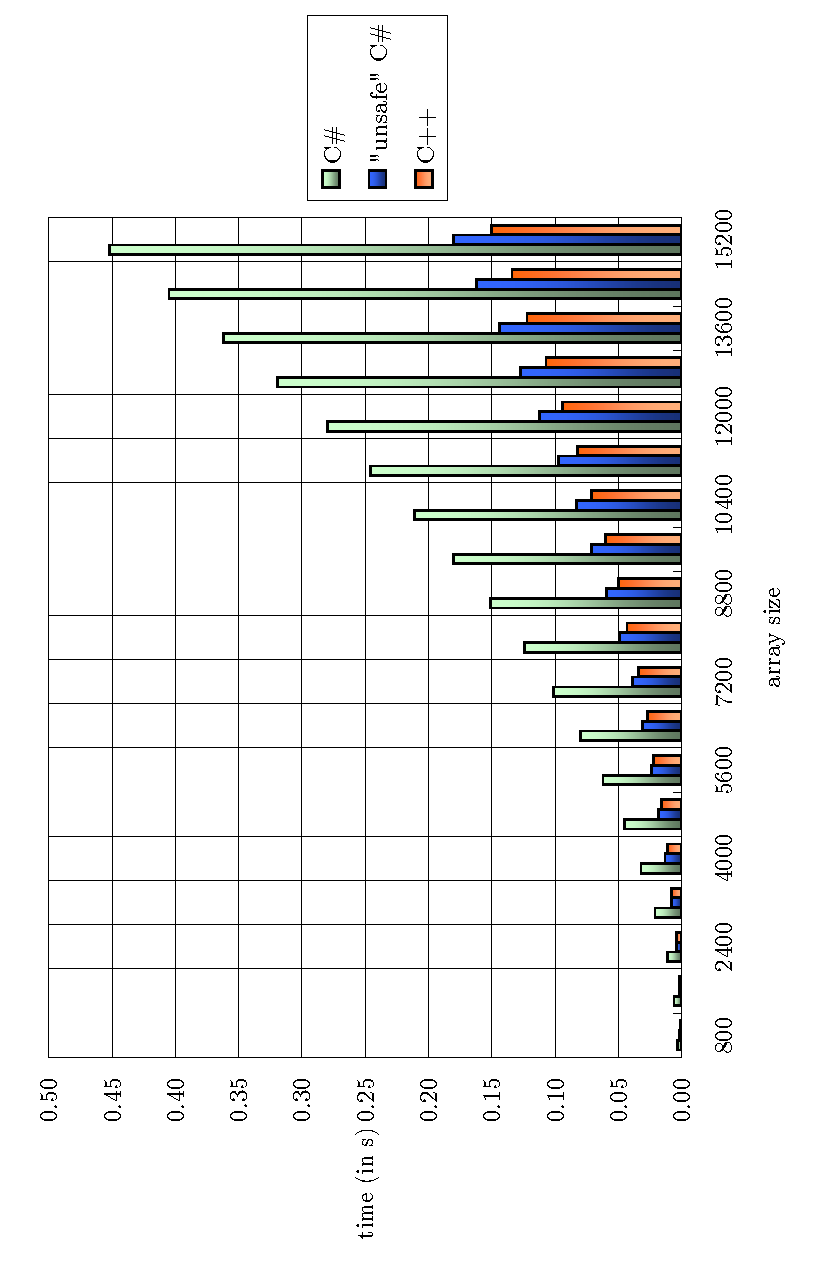
\includegraphics[width=9cm,angle=-90]{graphics/laboratory/00-langcomparison.pdf}
\caption{Results of \cpp vs. \csharp comparison}\label{figure:comparison}
\end{figure}

We see that \cpp outperformed classic \csharp implementation, while being a\-round 3 times faster. Even \enquote{unsafe} \csharp implementation got beaten, although the difference was tiny. So we can state that \cpp is faster than \csharp even in fairly simple task. You may think about performance difference if hugely complex computation (perhaps some 3D graphical computation) is needed to be done.

\item[HUGE COMMUNITY\ts{\textcolor{YellowOrange}{great}}]\hfill \\
Plenty of world-renowned software is written using \cpp{}, including many 3D games, almost each program from Adobe and Chromium web browser. Many \cpp books are available, making it easier to learn.

\fdocabbrevdeclare{JRE}{JRE}{Java Runtime Environment}
\item[MEMORY CONSUMPTION\ts{\textcolor{ultragreen}{good}}]\hfill \\
\cpp applications, as stated, need no virtual machine for their execution. They load just base \cpp library and extra libraries if needed. Such approach makes significant opposite to robust and greedy (as for memory) runtime environments of certain high-level languages. We can mention primarily .NET Framework and \fdocabbrevref{JRE}.

\item[CODE PORTABILITY\ts{\textcolor{red}{bad}}]\hfill \\
When it comes to code portability (same as multi-platformity), \cpp leaves its audience uncertain. Users can be sure about portability of \cpp standard library but that's all. Standard library is not trully packed with stunning features, forcing you to use \nth{3}-party libraries for advanced functionality. Those libraries don't have to be multi-platform, however, which can result in pain rooting from hypothetical need to port your application to another platform.

\item[MISSING CONSTRUCTS\ts{\textcolor{red}{bad}}]\hfill \\
Indeed, \cpp might be missing some very useful language constructs, which are quite common in other (\eg functional, logic or perhaps declarative) programming paradigms. Many features emerged in \cpp11 revision, however.
\end{description}

\vfill

\subsection{Version 11 and its enhancements}
\cpp programming language was, for the first time, standardized in 1998. This version is known as \cpp98 and if someone talks about \cpp, he probably has this version in mind. Programming was changing depending on time and so \cpp had to change to catch new trends and demands of its users.

\cpp11 brought many new features, eliminating some of its annoyances. You can read about \cpp11 in a massively extensive \citep{various:cppstandard} or goe through its finest new properties right now. It is recommended to know something about \cpp11 as its support is turned on in Qt 5 by default on supported compilers.

\subsubsection{Basic C plus plus 11 information}
\cpp11 is source code compatible with C and with \cpp98. It means that valid C (or \cpp98) source code is valid \cpp11 code too. Inprovements in \cpp were done in two categories: language core and standard library.

\paragraph{Language core improvements}
Syntax of \cpp was always considered to be evil, which is partially true, because \cpp offers huge collection of syntactical constructs and sugar, compared to other well-known programming languages. Moreover, \cpp11 adds new language constructs.

\paragraph*{Compile time constants}
In \cpp98, you cannot write some thing like:
\begin{lstlisting}[firstnumber=1,language=cpp]
int happy_number() {
	return 7;
}
int *array = new array[10];
array[happy_number()] = happy_number();
\end{lstlisting}
In this case, compilation ends with error saying: \enquote{Function \fdocinlinecode{cpp}{!}{happy_number()} is not a constant expression.} But you think it is. It returns $7$ everytime it's called, so it actually is constant expression. That's true but compiler is not aware of it. Keyword\fdocinlinecode{cpp}{!}{constexpr} tells the compiler to regard\fdocinlinecode{cpp}{!}{happy_number()} as constant expression, resulting in this code:
\begin{lstlisting}[firstnumber=1,language=cpp]
constexpr int happy_number() {
	return 7;
}
int *array = new array[10];
array[happy_number()] = happy_number();
\end{lstlisting}

\paragraph*{Initializer lists}
Consider having the custom class which encapsulates\fdocinlinecode{cpp}{!}{std::list} and perhaps adds some functionality:
\begin{lstlisting}[firstnumber=1,language=cpp]
class CustomList {
	private:
		std::list<int> m_list;
	
	public:
		CustomList();
		
		void insert(int i) {
			m_list.push_back(i);		
		}
};
\end{lstlisting}
Such an implementation allows you to instantiate empty\fdocinlinecode{cpp}{!}{CustomList} and fill it with values one by one via\fdocinlinecode{cpp}{!}{insert(int i)} method. But what if you know all values in compile time? In older \cpp you would have to insert all values one by one. (Note that there is no\fdocinlinecode{cpp}{!}{CustomList(const std::list &list)} constructor available.) But \cpp11 allows you to use initializer list:
\begin{fdoccode}{cpp}{listing:initializer}{Initializer list usage}
class CustomList {
	private:
		std::list<int> m_list;
	
	public:
		CustomList();
		CustomList(std::initializer_list<int> values) {
			for (int &value : values) {(*@\label{listing:forloop}@*)
				m_list.push_back(value);			
			}
		}
		
		void insert(int i) {
			m_list.push_back(i);		
		}
};

// Creating CustomList instance and filling it with values.
CustomList my_list_instance = {1, 2, 3, 4, 5, 6, 7};
\end{fdoccode}

\paragraph*{Clever for-loops}
Careful reader certainly noticed strange notation of for-loop in \autoref{listing:initializer} on line \ref{listing:forloop}. This new for-loop syntax is known as \textit{range-based for-loop}.\footnote{This kind of for-loop is available in Qt too, as we will see later.} It's just syntactical sugar. This loop works for all containers in standard library as well as for classic C-style arrays. Furthermore, all custom containers defining its iterators are supported too.

\paragraph*{Type deduction}
\cpp is statically typed language. So you, as programmer, have to know and mark the type of each and every variable you declare. You basically write:
\begin{lstlisting}[firstnumber=1,language=cpp]
int variable_1 = 15;
std:list<int> *variable_2 = new std::list<int>();
\end{lstlisting}
or something similar. \cpp11 allows you to omit type of variable with the\fdocinlinecode{cpp}{!}{auto} keyword:
\begin{lstlisting}[firstnumber=1,language=cpp]
auto variable_1 = 15;
auto *variable_2 = new std::list<int>();
\end{lstlisting}
Compiler deduces type of each \enquote{automatic} variable during compilation. This feature is useful when that particular type is hard to write.\footnote{\cpp programmers used to use\fdocinlinecode{cpp}{!}{typedef} to \enquote{clone} types and assign shorter names to them.} You can use\fdocinlinecode{cpp}{!}{auto} in every thinkable situation as compiler does type checking anyway. Automatic type deduction works for pointer types too.

\paragraph*{Lambda expressions}
Well, lambda expressions were the most expected feature. Known from functional languages (\eg Common Lisp, Scheme), they rapidly penetrated even object-oriented programming. Lambda expressions\index{lambda expression} are basically function objects. They can have input parameters and return values.

Lambdas are functions which are defined within another function, thus having no identifier. Typical lambda expression looks like this:
\begin{lstlisting}[firstnumber=1,language=cpp]
[] (int input_1, int input_2) -> int {
	return input_1 * input_2;
}
\end{lstlisting}
Tricky thing is that lambda expression is able to use variables from the \enquote{outside} of its body. Lambdas can be assigned to automatic variable and user can even decide if he (or she) wants to allocate lambda expression on the stack\index{stack} or on the heap\index{heap}:
\begin{lstlisting}[firstnumber=1,language=cpp]
auto twice_function_stack = [] (double input_1) -> double {
	return input_1 * double;
};

auto twice_function_heap = new auto ([] (double input_1) -> double {
	return input_1 * double;
});
\end{lstlisting}
Lambda expression can be used as function parameter too. Very simple (and kind of naive) implementation of in-place map function can look like the on in \autoref{listing:lambda}.
\begin{fdoccode}{cpp}{listing:lambda}{Lamda expression as function parameter}
#include <iostream>
#include <functional>
#include <list>


// In-place map function.
// Executes func for each member of input_list
void map(const std::function<void(double&)> &func, std::list<double> &input_list) {

    // Range-based for-loop.
    for (double &value : input_list) {
		func(value);
    }
}

int main(int argc, char *argv[]) {
    // Create simple list using list initializer.
    std::list<double> my_list = {1.7, 2.8, 4.9, 5.9, 0.0};

    // Instantiate lambda expression (anonymous function).
    auto func_twice = [&] (double &input) {
		input *= 2;
    };

    // Use lambda expression as function parameter.
    map(func_twice, my_list);

    for (double value : my_list) {
		std::cout << value << " ";
    }
    return 0;
}
\end{fdoccode}
Lambda expressions make huge impact on Qt 5.

\paragraph*{Null pointers}\index{null}\index{pointer}
It is quite common to type something like\fdocinlinecode{cpp}{!}{int *variable = NULL} in \cpp03. Let's expand\fdocinlinecode{cpp}{!}{NULL}. In most cases, the result is\fdocinlinecode{cpp}{!}{#define NULL ((void *)0)}. So\fdocinlinecode{cpp}{!}{NULL} is literally \enquote{the pointer pointing to nothing of any possible type.}

Problem occurs if\fdocinlinecode{cpp}{!}{NULL} is defined as $0$. Troubles might appear when overloaded function gets called with such a\fdocinlinecode{cpp}{!}{NULL}. It's not obvious if\fdocinlinecode{cpp}{!}{function(int)} or\fdocinlinecode{cpp}{!}{function(int*)} gets called by\fdocinlinecode{cpp}{!}{function(variable)}. It might be the first function on one system or second one on another system.

\cpp11 implements new keyword\fdocinlinecode{cpp}{!}{nullptr} wich is always evaluated to correct value.

\paragraph{Standard library improvements}\index{standard library}
Standard library has always been quite tiny. It included just necessary classes, nothing special. But time goes forward, so that standard library must too. Number of fine classes were added.

\paragraph*{Threading}\index{thread}
Finally, threading was introduced within the standard library. This threading subsystem should not depend on operating system threading implementation. But threading-related stuff in Qt depends on specific classes from operating system (pthreads on Linux)\index{pthreads}\index{Linux} and work really fine. So these standardized threading facilities are not so important for ordinary Qt user.

\paragraph*{Tuples (pairs)}\index{tuple}
Good bonus for every \cpp programmer. No need to use \nth{3} party tuples implementations. More classes are new in the standard library, look at \citep{various:cppstandard} for more.

\section{Qt components}\label{section:components}
Qt consists of libraries, tools and other supplemental software. You have already seen very brief list of Qt components in \autoref{section:what}. Libraries themselves are divided into so-called \textit{modules}\index{modules}.\footnote{You are not familiar with modules yet. Module is simply collection of related classes.} You can learn more about modules in \autoref{section:qtstructure}. Let's look into Qt library collection more thoroughly. Qt library collection contains these main components:
\begin{enumerate}
\item Tools for \fdocabbrevref{GUI} design and implementation consisting of user interface designer (QtDesiger) and user interface classes (known as QtWidgets and QtGui).
\item Painting system which is accessory for \fdocabbrevref{GUI} design or can server as the main force for creating graphics-related software, \eg painting applications, video editors or perhaps chart designer programs.
\item Testing facilities which enable you to use test-driven development model. Unit-testing is extremely useful for large-scaled projects.
\item Complete thread subsystem that allows you to split your application computations among several threads of execution, making your program more robust and versatile.
\item Networking machinery for swift network communication between workstations and even among processes or threads.
\fdocabbrevdeclare{MVC}{MVC}{Model-view-controller}
\item \fdocabbrevref{MVC} architecture for binding your data to \fdocabbrevref{GUI} or for structuring your data for further usage via abstraction layer (data model).
\item Resource system which allows you to embed any file directly into executable file, including pictures, music files or text files.
\fdocabbrevdeclare{XML}{XML}{Extensible Markup Language}
\item Facilities for \fdocabbrevref{XML} manupilation, web services integration, integrated help mechanisms, printing support, OpenGL wrapper, vector graphics classes, \ldots
\end{enumerate}

Some parts from this (not-so-complete) list will be examined deeply, some won't.

\subsection{Supported platforms}
Qt 5 is multi-platform framework and support of various operating systems and platforms is one if its key features if now the biggest one. Supported operating systems are:
\begin{itemize}
\item Windows ($+$ Windows Embedded Compact)
\item Linux
\item Mac OS X
\item OS/2 (eComStation)
\item Android (via Necessitas port)
\end{itemize}
Qt is ported to even more operating systems but those ports lack quality and completeness.

\subsection{Qt 5 additions}
Qt 5 concetrates on using modern technologies for painting user interfaces and introduces many other tweaks and improvements:
\begin{itemize}
\item
Qt 5 is neither binary nor source code compatible with previous Qt releases, resulting in need of refactoring and recompilation of your Qt 4-based applications. You can blame Digia for bad approach but it's better not to compromise sometimes. Qt 3 support was dropped too.

\fdocabbrevdeclare{QPA}{QPA}{Qt Platform Abstraction}

\item
Brand new Qt component named \fdocabbrevref{QPA}, allowing you to easier port Qt 5 for new platform and operating systems.

\item
All classes were update to conform to Unicode 6.2 standard.

\item
Quite important change happened in the QtGui\index{QtGui} module as all widget classes got moved into newly established QtWidgets\index{QtWidgets} module.

\item
QtQuick\index{QtQuick} made it to version 2. QtQuick is module for writing applications using \fdocabbrevref{QML}.

\item
QtWebKitWidgets\index{QtWebKitWidgets} now includes rewritten Webkit-based\index{Webkit} html rendering engine. Html 5, Canvas and WebGL are supported and web pages are now fetched asynchronously.

\fdocabbrevdeclare{GCC}{GCC}{GNU Compiler Collection}
\fdocabbrevdeclare{MSVC}{MSVC}{Microsoft Visual \cpp}

\item
\cpp98 -- 11 compilers are supported.\footnote{Note that some compilers (\eg \fdocabbrevref{MSVC} compiler) do not support all \cpp11 features yet. Use acclaimed \fdocabbrevref{GCC} in case of problems.} Meta-object system was tweaked too and you will be informed about those changes later.

\item
New multi-platform user interface style called Fusion is available (\autoref{figure:fusion}).
\end{itemize}

\begin{figure}[ht]
\centering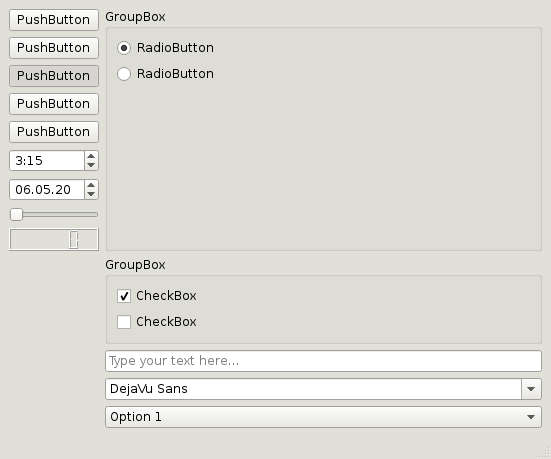
\includegraphics{graphics/laboratory/01-fusion.png}
\caption{Qt Fusion style example}\label{figure:fusion}
\end{figure}

\section{Getting and installing Qt}
There are basically three ways of obtaining Qt framework:
\begin{enumerate}
\item You have bought commercial Qt license so you can use specific Qt packages provided by Digia.
\item You can download open-source Qt framework directly from \href{http://www.qt-project.org/}{www.qt-pro\-/ject.org}.
\item You use a Linux distribution which can equip you with Qt framework via some kind of native packaging system.
\end{enumerate}

Qt can be downloaded as executable installer file which containes binaries precompiled for you as well as documentation and other needed tools. Sometimes manual compilation is needed.\footnote{It is commonly known that Qt compilation can last for several hours. Thus, consider getting precompiled binaries instead of compiling those by yourself.}

Qt framework versions gets released precompiled for certain compilers only. Linux releases are meant to work with \fdocabbrevref{GCC}, Windows releases are usually precompiled by \fdocabbrevref{MSVC}. Qt framework with MinGW support is released from time to time too.

\subsection{Installing Qt on Windows}
%% instalace na windows a linuxu
Qt installation on Windows is fairly straightforward if binaries are available. All you need to do is obtain the setup executable file and follow instructions. Some troubles might occur, though.

Let's assume that Qt was installed in\fdocinlinecode{text}{!}{c:\\Qt\\Qt5.0.0\\}.

You need to tweak your PATH environment variable in order to be able to run Qt tools from command line. Qt Creator will work even without proper PATH because it does all necessary settings for itself automatically. You can setup PATH variable in Windows 7 as follows:
\begin{enumerate}
\item From the desktop, right-click (by mouse) \enquote{My Computer} and then click \enquote{Properties}.
\item Choose \enquote{Advanced System Settings} from the list.
\item In the \enquote{System Properties} window, hit the \enquote{Environment Variables} button.
\item Locate \enquote{System variables} group, select PATH variable and hit \enquote{Edit} button.
\item Move to the end of the string and add folowing paths:
\begin{lstlisting}[firstnumber=1,language=text]
c:\Qt\Qt5.0.0\5.0.0\msvc2010\bin\
c:\Qt\Qt5.0.0\Tools\QtCreator\bin\ (If Qt Creator is installed too.)
\end{lstlisting}
Paths within the PATH variable are separated by semicolons. Typical content of PATH variable may look like the one in \autoref{listing:pathwindows}.
\begin{fdoccode}{text}{listing:pathwindows}{Setting PATH environment variable for Qt on Windows}
%SystemRoot%\system32;%SystemRoot%;c:\Qt\Qt5.0.0\5.0.0\msvc2010\bin\;c:\Qt\Qt5.0.0\Tools\QtCreator\bin\
\end{fdoccode}
\end{enumerate}

\subsection{Installing Qt on Linux}
As stated, Qt can be installed on Linux in two ways:
\begin{enumerate}
\item Linux distribution \textit{package manager}\index{package manager} offers it as the package. This is the case for many major distributions, \eg Ubuntu, Archlinux, Fedora, Debian or Mint.
\item Classical installation via executable file:
\begin{enumerate}
\item Obtain installation file from \href{http://www.qt-project.org/}{www.qt-pro\-/ject.org}.
\item Open terminal\index{terminal} and navigate to folder containing obtained installation file.
\item Change permissions on the file:
\begin{lstlisting}[firstnumber=1,language=text]
sudo chmod +x ./qt-5-installation-file.run
\end{lstlisting}
You need to run\fdocinlinecode{text}{!}{chmod} as superuser\index{superuser} (root\index{root}) if you want to install Qt into system-wide location.

\item Install Qt by executing\fdocinlinecode{text}{!}{./qt-5-installation-file.run}, follow on-screen instructions. It's good to install Qt into separate folder structure to keep system structure clean. Using\fdocinlinecode{text}{!}{/opt/qt5} as base installation directory is generally good idea.

\item There is no need of editing PATH environment variable if you use Qt Creator for development. Otherwise, make sure you set correct values to environment variables (see \autoref{listing:pathlinux}).
\begin{fdoccode}{text}{listing:pathlinux}{Setting environment variables for Qt on Linux}
QTDIR=/opt/qt5/5.0.0/gcc
PATH=$PATH:$QTDIR/bin
QMAKESPEC=$QTDIR/mkspecs/linux-g++
\end{fdoccode}
\fdocinlinecode{text}{!}{QTDIR} variable contains path to root qt directory. This is the directory which contains subdirectories\fdocinlinecode{text}{!}{bin},\fdocinlinecode{text}{!}{include},\fdocinlinecode{text}{!}{lib}, \ldots
\end{enumerate}
\end{enumerate}


\subsection{Compilling Qt}\index{compilation}
Sometimes, you may need to compile Qt on your own. Compilation allows you to throw away features you do not like, resulting in smaller dynamic (and static too) libraries sizes.

Qt sources are always contained within compressed file. All you need to do is to have correctly installed \cpp compiler (\fdocabbrevref{GCC} or \fdocabbrevref{MSVC} are recommended). Basic compilation steps are quite similar for each operating system:
\begin{enumerate}
\item Decompress source package and navigate to its root folder using terminal (command prompt).
\item Run\fdocinlinecode{text}{!}{./configure -opensource -nomake examples -nomake tests}.
\item Now, run\fdocinlinecode{text}{!}{make} (on Linux),\fdocinlinecode{text}{!}{nmake} (on Windows with Visual Studio) or\fdocinlinecode{text}{!}{mingw32-make} (on Windows with MinGW).
\end{enumerate}

Compilation process can be long and painful, as many problems can occur. See \citep{various:qtdoc} for more information.
\section{Qt framework structure}\label{section:qtstructure}
Qt framework itself is a huge software collection and needs to be divided into logical units. Two main units are \textit{libraries} and \textit{additional software}.

Additional software includes compilers, tools for internationalization and tens of other tools. Some of them will be described in \autoref{section:compilation}.

Let's dig into Qt libraries now. Qt offers very rich and diverse functionality (see \autoref{section:components}), ranging from network communication to painting vector pictures.

\subsection{Modules}
Each unit of related functionality is called \textit{module}\index{module}. Module is set of classes which is contained within the single (static or dynamic, see \autoref{section:compilation}) library file. If you want to use this module in your code, then you have to include appropriate header files and link your binary against the library file. More modules you need results in more linked libraries and bigger output binaries. Choice of Qt modules for application programming is therefore important.

\begin{fdocextra}
There are two types of library linkage:
\begin{description}
\item[DYNAMIC LINKAGE] \hfill \\
Is very popular for its usefulness. Dynamic linking\index{dynamic linkage} means that executable file (operating system more precisely) seeks for needed libraries in certain predefined paths in run time. Usually one version of each library is placed somewhere in well-known folder structure and each executable is linked against it. So more running executables can actually use the same library file. This saves memory and is very popular within Unix-like operating systems but it can bring certain level of disorder into poorly designed operating system. This has something to do with Windows because many applications doesn't link with libraries stored in system path and use varying versions of the same library sometimes, duplicating library presence in memory and increasing memory usage.
\item[STATIC LINKAGE] \hfill \\
Not so favourite kind of linkage. Library is packed into executable file and linked in compile time. This makes executable file (sometimes considerably) larger but no additional dependencies (in form of external dynamic libraries) are required. GNU GPL\index{GNU GPL} Qt libraries \textbf{cannot} be linked statically.
\end{description}
\end{fdocextra}

\subsubsection{Linking}
Each module usually depends on QtCore\index{QtCore} module, including QtWidgets module. Moreover, QtWidgets module depends on QtGui module. So each Qt-based application with user interface has to be linked against 3 or more modules.

Consider elementary \fdocabbrevref{GUI} application with main window. You can find source in\fdocinlinecode{text}{!}{sources/laboratory/04-guiapp} subdirectory. Application is compiled with modules QtCore and QtWidgets. You can use GNU \textit{ldd}\index{ldd} application to list all dynamic libraries required for executable file to run successfully. Output for our sample application looks very similar to the on in \autoref{listing:ldd}.

\begin{fdoccode}{text}{listing:ldd}{Libraries needed for \fdocabbrevref{GUI} application}
[root@arch-linux 04-guiapp]# ldd -d -r 04-guiapp
linux-gate.so.1 (0xb77c7000)
libQt5Widgets.so.5 => /opt/qt5/5.0.0/gcc/lib/libQt5Widgets.so.5 (0xb719f000) (*@\label{listing:qt5w}@*)
libQt5Gui.so.5 => /opt/qt5/5.0.0/gcc/lib/libQt5Gui.so.5 (0xb6d89000)
libQt5Core.so.5 => /opt/qt5/5.0.0/gcc/lib/libQt5Core.so.5 (0xb693f000) (*@\label{listing:qt5c}@*)
libGL.so.1 => /usr/lib/libGL.so.1 (0xb6833000)
libpthread.so.0 => /usr/lib/libpthread.so.0 (0xb6817000)
libstdc++.so.6 => /usr/lib/libstdc++.so.6 (0xb672e000)
libm.so.6 => /usr/lib/libm.so.6 (0xb66eb000)
libgcc_s.so.1 => /usr/lib/libgcc_s.so.1 (0xb66ce000)
libc.so.6 => /usr/lib/libc.so.6 (0xb651d000)
libgobject-2.0.so.0 => /usr/lib/libgobject-2.0.so.0 (0xb64cd000)
libglib-2.0.so.0 => /usr/lib/libglib-2.0.so.0 (0xb63d2000)
libX11.so.6 => /usr/lib/libX11.so.6 (0xb629c000)
libicui18n.so.49 => /opt/qt5/5.0.0/gcc/lib/libicui18n.so.49 (0xb6084000)
libicuuc.so.49 => /opt/qt5/5.0.0/gcc/lib/libicuuc.so.49 (0xb5f0a000)
libdl.so.2 => /usr/lib/libdl.so.2 (0xb5f05000)
libgthread-2.0.so.0 => /usr/lib/libgthread-2.0.so.0 (0xb5f01000)
librt.so.1 => /usr/lib/librt.so.1 (0xb5ef8000)
/lib/ld-linux.so.2 (0xb77c8000)
libXext.so.6 => /usr/lib/libXext.so.6 (0xb5ee5000)
libpcre.so.1 => /usr/lib/libpcre.so.1 (0xb5e7d000)
libffi.so.6 => /usr/lib/libffi.so.6 (0xb5e76000)
libxcb.so.1 => /usr/lib/libxcb.so.1 (0xb5e53000)
libicudata.so.49 => /opt/qt5/5.0.0/gcc/lib/libicudata.so.49 (0xb4d32000)
libXau.so.6 => /usr/lib/libXau.so.6 (0xb4d2e000)
libXdmcp.so.6 => /usr/lib/libXdmcp.so.6 (0xb4d27000)
\end{fdoccode}

Pay attention to lines \ref{listing:qt5w} -- \ref{listing:qt5c}. Typical program with user interface needs to be linked against QtCore, QtGui and QtWidgets. Console applications need just QtCore.

You can list unused (but linked) libraries too as seen in \autoref{listing:ldd2}.

\begin{fdoccode}{text}{listing:ldd2}{Unused (but linked) libraries for \fdocabbrevref{GUI} application}
[root@arch-linux 04-guiapp]# ldd -d -r -u 04-guiapp
Unused direct dependencies:
/opt/qt5/5.0.0/gcc/lib/libQt5Gui.so.5
/usr/lib/libGL.so.1
/usr/lib/libpthread.so.0
/usr/lib/libm.so.6
\end{fdoccode}

Threading library (pthread\index{pthread}) is used by QtCore on Linux. LibGL\index{libGL} is 3D graphics library. LibGL is unused because no OpenGL-related\index{OpenGL} function was called explicitly in our sample application. You will learn more about linking in \autoref{section:compilation}.

\subsection{Tree-like class structure}
Cleverly developed library has smart class structure which makes that library easily maintainable, expandable and functional. \textit{Class inheritance}\index{class inheritance} is used very extensively if library design is something we need to deal with. Read \citep[p.~708-783]{prata:cprimer} to get more familiar with \cpp class inheritance if you are not so far. Class inheritance says that if one class is inheritor of another class, then it inherits parent's \textit{data} and \textit{methods}.

It's good practice to have some properties available in all classes of the library. Such a property could be \eg \textit{id}, the textual (or perhaps numerical) identification of each object (instantiated class) within the library. You would have to define what \textit{id} means in each and every of your classes manually without inheritance usage. With inheritance, everything you must do, is to define \textit{id} in exactly one of your classes, promoting this class to \textit{root} class and make rest of classes to inherit the new \textit{library base class}.

This approach is good base to have library with the tree-like structure (see \autoref{figure:library}) where classes are structured according to their natural relationship.

\begin{fdocextra}
Many well-known libraries follow root class idea and tree-like class structure. One example is .NET Framework. Its very base class is called\fdocinlinecode{csharp}{!}{System.Object} and provides some basic functionality (shared by all .NET classes via class inheritance) such as method providing basic string representation of each object. You can find more about .NET base class in \citep[p.~84]{nigel:csharp}. Java follows very similar class hierarchy ideas.
\end{fdocextra}

\begin{figure}[ht]
\centering
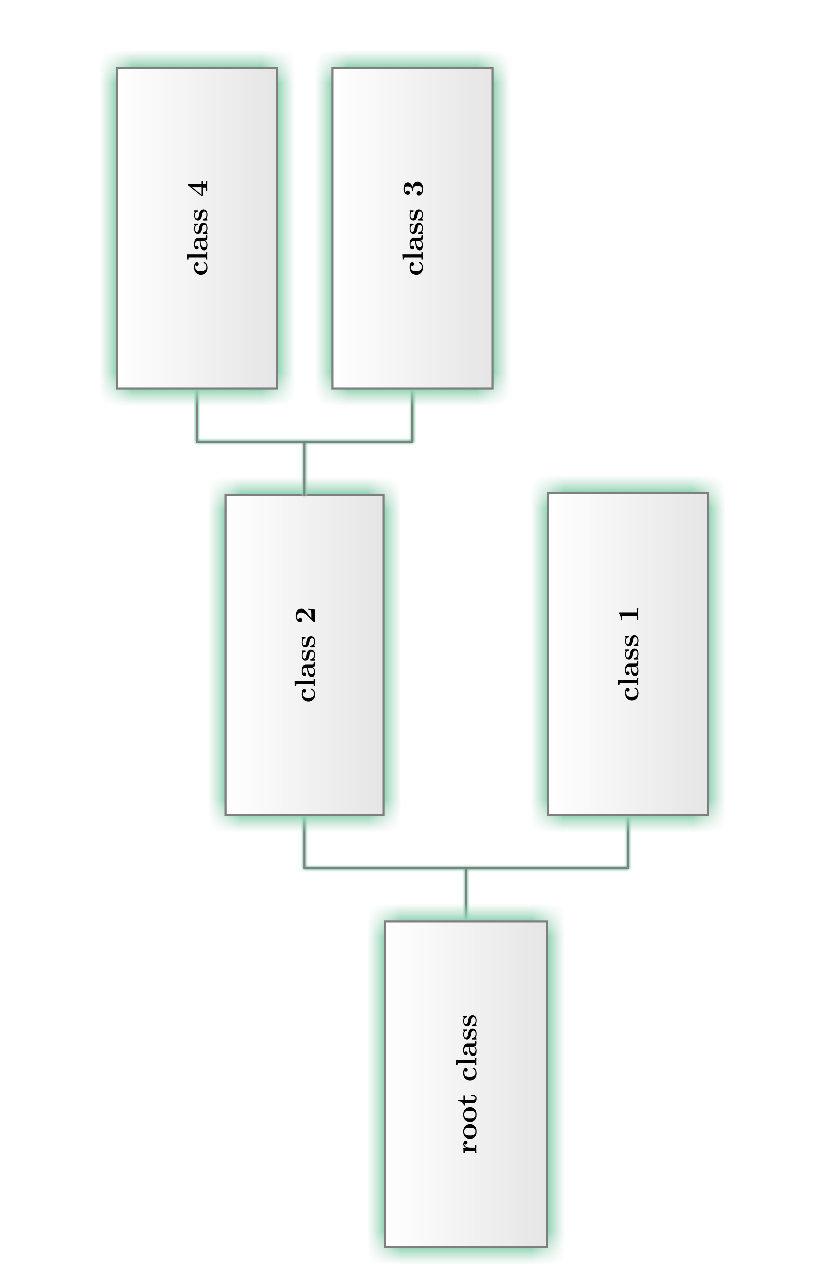
\includegraphics[angle=-90,width=12cm]{graphics/laboratory/02-tree.pdf}
\caption{Typical library tree-like class structure}\label{figure:library}
\end{figure}

So, as we found out, there is exactly one class that sits above other classes, which share its data and methods. Qt disposes this kind of top-level class too, it's called\fdocinlinecode{cpp}{!}{QObject}.
\chapter{Using Qt framework}
Basic Qt library structure is known to us but we need to know something about Qt-related development environments and tools. You can develop Qt applications in any development environment, including Microsoft Visual Studio\index{Visual Studio}. Some tools are part of Qt framework, however. This includes young and thriving Qt Creator\index{Qt Creator} development environment.

Every Qt/\cpp{} programmmer should be aware of existence of certain rules concerning source code appearance. These rules are called \textit{conventions}\index{convention} and you will learn about them too.

\section{Qt Creator}
Qt Creator (see \autoref{figure:qtcreator}) is fully-featured \cpp{} \& JavaScript development environment. It is suitable for plain \cpp{}  development as well as for Qt development. Qt Creator is part of Qt SDK, thus can be installed along with Qt libraries. Qt Creator supports big collection of features:\index{CMake}\index{Autotools}\index{QMake}
\begin{itemize}
\item multiple build systems (CMake, Autotools and QMake),
\item syntax highlighting for more than one hundred programming languages,
\item auto-completion for variables, functions and macros (see \autoref{figure:qtcreatorauto}),
\item consistent look on every supported operating system,
\item many plugins,
\item refactoring facilities,
\item tools for debugging,
\item cooperation with Android SDK,
\item dynamic keyboard shortcuts,
\item integrated Qt help system (see \autoref{figure:qtcreatorhelpfull}),
\item context-aware help (see \autoref{figure:qtcreatorhelp}),
\item support for simultaneously installed Qt frameworks,
\item integrated Qt Designer for \fdocabbrevref{GUI} design,
\item sharing source code via online services and many other features.
\end{itemize}

\begin{figure}[ht]
\centering
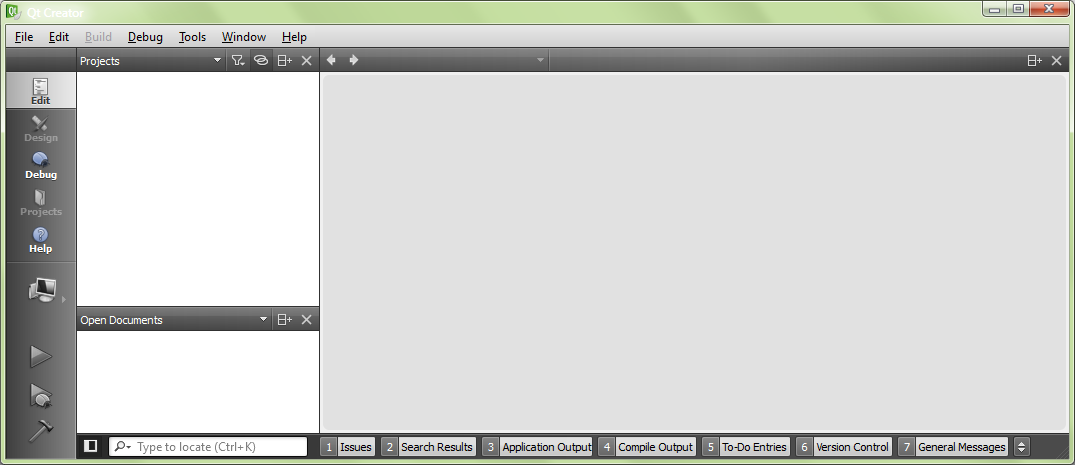
\includegraphics[width=14.5cm]{graphics/laboratory/03-qtcreator.png}
\caption{Qt Creator empty environment}\label{figure:qtcreator}
\end{figure}

\begin{figure}[ht]
\centering
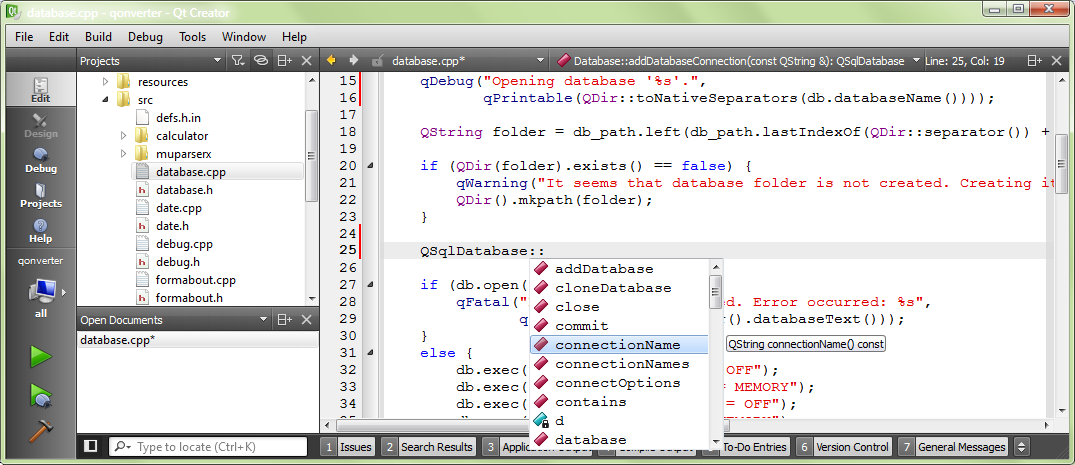
\includegraphics[width=14.5cm]{graphics/laboratory/04-qtcreator-auto.png}
\caption{Qt Creator auto-completion}\label{figure:qtcreatorauto}
\end{figure}

\begin{figure}[ht]
\centering
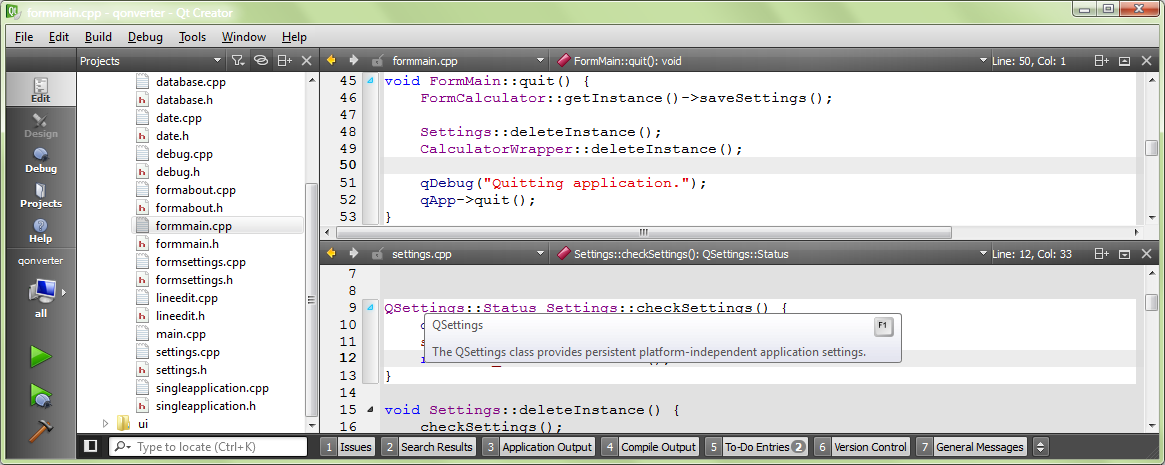
\includegraphics[width=14.5cm]{graphics/laboratory/05-qtcreator-help.png}
\caption{Qt Creator context-aware help}\label{figure:qtcreatorhelp}
\end{figure}

\begin{figure}[ht]
\centering
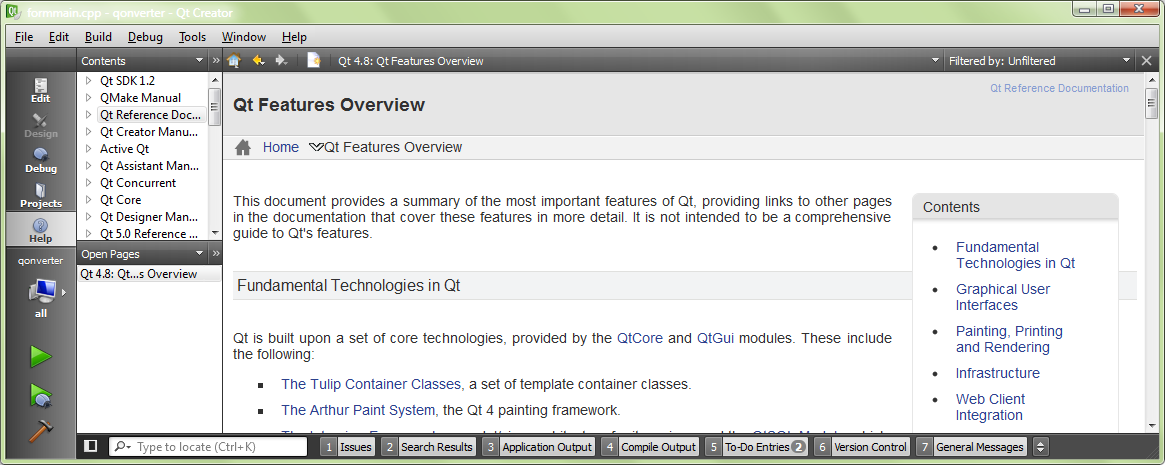
\includegraphics[width=14.5cm]{graphics/laboratory/06-qtcreator-help-full.png}
\caption{Qt Creator full reference documentation}\label{figure:qtcreatorhelpfull}
\end{figure}

\subsection{Speeding-up Qt Creator}
You can make Qt Creator less memory-hungry by disabling some unneeded plugins. You can disable plugins in\fdocinlinecode{text}{!}{About -> About Plugins...} menu. Minimal setup for desktop Qt development using CMake may look like the one in \autoref{table:plugins}.

\begin{table}[ht]
\begin{center}
\caption{Qt Creator minimal plugins setup}\label{table:plugins}
\begin{tabular}{c | c}
enabled & disabled \\
\hline
CMakeProjectManager & AutotoolsProjectManager \\
GenericProjectManager & ClassView \\
Qt4ProjectManager & CodeAnalyzer \\
QtSupport & DeviceSupport \\
CppEditor & GLSL \\
CppTools & BinEditor \\
Debugger & Bookmarks \\
Designer & ImageViewer \\
Help & Macros \\
ProjectExplorer & UpdateInfo \\
ResourceEditor & Welcome \\
CodePaster & QtQuick \\
Todo & FakeVim \\
 & HelloWorld \\
 & TaskList \\
 & VersionControl 
\end{tabular}
\end{center}
\end{table}

\section{Qt Designer}
Qt Designer\index{Qt Designer} (see \autoref{figure:designer}) is a tool for user interface design. It is standalone application which is integrated into Qt Creator too.

\begin{figure}[ht]
\centering
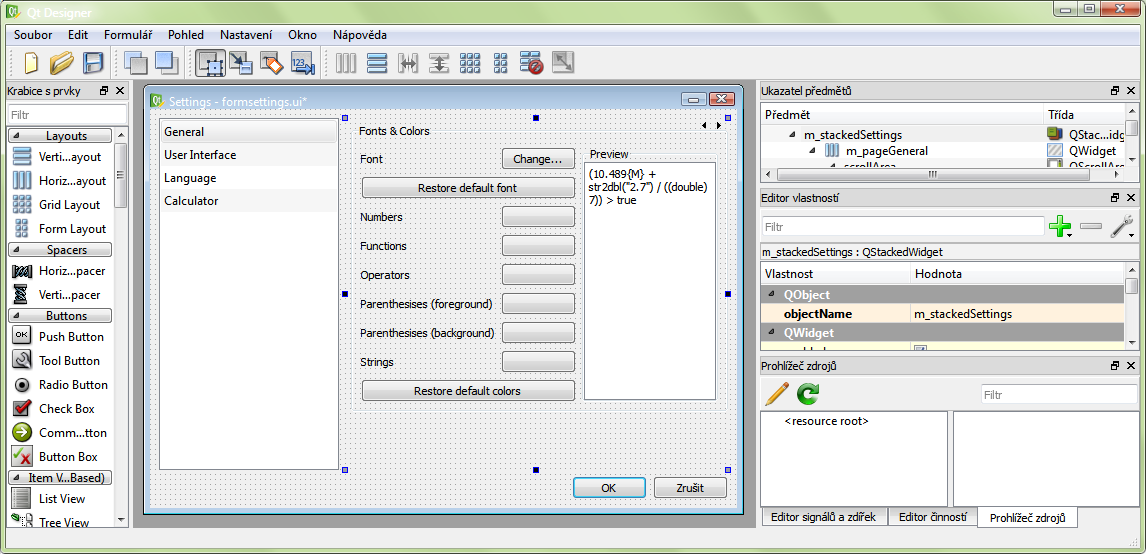
\includegraphics[width=14.5cm]{graphics/laboratory/07-designer.png}
\caption{Qt Designer environment}\label{figure:designer}
\end{figure}

\section{Tools and chains}
Qt Creator supports multiple compilers and multiple Qt libraries installed side by side. You can choose any installed compiler or Qt library to build your projects. Qt Creator uses special terminology for groups of compilers and Qt libraries called \textit{kits}. Kit (see typical kit setup in \autoref{figure:kit}) is virtual container for one compiler and one specific Qt library (for example Qt 5 library). Moreover, kit specifies primary debugger and other stuff needed to compile your projects. Kit (or \textit{toolchain}) says what is used to compile your project. You can manage compilers and Qt versions in\fdocinlinecode{text}{!}{Build & Run} section of Qt Creator settings dialog.

\begin{figure}[ht]
\centering
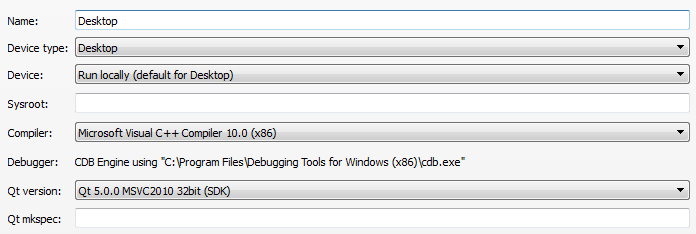
\includegraphics[width=11cm]{graphics/laboratory/08-qtcreator-kits.png}
\caption{Qt Creator kit setup}\label{figure:kit}
\end{figure}

\section{Code conventions}
Writing working application is not enough in Qt world. Qt itself is huge library and rules are more important here than everywhere. These rules we talk about apply primarily to our source code. Code must be self-descriptive. This can be achieved by following certain code conventions. We are talking here about source code \enquote{typography}.\footnote{You should assure yourself you have some base to build on before you proceed. If certainty is not solid, then take a look at \citep[p.~40-77]{mcconnell:codecomplete}.}

\subsection{What are conventions?}
Programming can be very difficult job sometimes. That's why programmers do need to make their work easier. Conventions are tools to achieve that. It's always useful to know what certain source code does simply by taking a brief look at it. If this happens, then code is written well, it is readable, understandable and it is actually joy to browse it.

Let's compare source code to formatted text (\eg{} text of a book). Good books do have their content formatted so that reader can read it smoothly and comfortably. It is supplemented with pictures, tables, charts and diagrams. Text itself is separated into paragraphs (usually one paragraph per idea), which can have indented first lines or can be separated by vertical white space. In addition, important words can be \textcolor{purple}{highlighted} with color or \emph{emphasised} alternatively. You can disagree with claims in this paragraph but these claims can be summed up into one thing called \emph{style}\index{style}. Your potential disagreement signs that there are many various styles. Some apply to books, other ones to cars. Styles are not perfect. If majority of interested people likes these adjustments (\eg visual adjustments of source code), then we call these adjustments a \emph{conventions}\index{convention}. Almost everything can have its style and conventions. Style makes things usable and predictable.

Good programmer has to realise he produces source code not for him but for other programmers in a community or in a team. Aware programmer produces code styled the way a team (or a community) likes, not the way that he wants.

\subsection{Applying Qt conventions}
Compare \autoref{listing:badstyle} and \autoref{listing:goodstyle}. Just a brief look can advise you what is meant by code readability.
\begin{fdoccode}{cpp}{listing:badstyle}{Bad code style}
#ifndef CAR_H
#define CAR_H

#include <QtCore/QDebug>


class Car {
    private:
		unsigned int NumberOfWheels;
    public:
		Car(int w);
		void showMeThisParticularCar();
    private:
		bool owner;
};
#endif // CAR_H
\end{fdoccode}

\begin{fdoccode}{cpp}{listing:goodstyle}{Good code style}
#ifndef CAR_H
#define CAR_H


class Car {
    public:
		// Creates new car.
		Car(int number_of_wheels, bool has_owner = true);

		// Displays information about this car.
		void showCar();

    private:
		int m_numberOfWheels; // Stores count of wheels of this car.
		bool m_hasOwner; // True if this cas is owned by someone.
};

#endif // CAR_H
\end{fdoccode}

There are considerable differences between these two code fragments. Conventions importance is not probably obvious because of code length but it will grow rapidly with regard to code complexity and length. We should examine lines of \autoref{listing:goodstyle} now.

\subsection{Elements of good Qt code style}
Base for \autoref{listing:goodstyle} is sample application in\fdocinlinecode{text}{!}{sources/laboratory/06-good-car}. Let's explore both file\fdocinlinecode{text}{!}{sources/laboratory/06-good-car/car.h} and\fdocinlinecode{text}{!}{sources/laboratory/06-good-car/car.cpp}.

\subsubsection*{File car.h}
Using two blank lines between header file last\fdocinlinecode{cpp}{!}{#define} macro and class declaration beginning is generally good habit. Some programmers use just one blank line.
\begin{lstlisting}[firstnumber=1,language=cpp]
#ifndef CAR_H
#define CAR_H


class Car {
\end{lstlisting}
Blank-lining is good in many constructs of \cpp language. One blank line should appear before each class section except the first one.
\begin{lstlisting}[firstnumber=5,language=cpp]
class Car {
    public:
\end{lstlisting}
Comment\index{code comment} your code. Comments are essential part of source code. Always comment parts of code which are not straightforward.
\begin{lstlisting}[firstnumber=7,language=cpp]
	// Creates new car.
\end{lstlisting}
Use lower-cased names for variables in functions (methods) with undersore as delimiter for words in a variable name. Boolean variables should include verb in its name.
\begin{lstlisting}[firstnumber=8,language=cpp]
	Car(int number_of_wheels, bool has_owner = true);
\end{lstlisting}
Note that method should contain verb in its name because method always \enquote{does} something. Sometimes, single verb as name is pretty enough to describe what method does or how it works. Use Camel notation\index{notations!Camel} for methods. In Camel notation, all words in a compound (except first word) begin with upper-case letter and are not separated by spaces or any other character.
\begin{lstlisting}[firstnumber=11,language=cpp]
	void showCar();
\end{lstlisting}
Use Hungarian notation\index{notations!Hungarian} for data members of each and every class. In Hungarian notation, all variable names have prefix which signals data type or purpose of the variable. It is recommended to delimite prefixes by underscore character. Members prefixed with\fdocinlinecode{cpp}{!}{m_} are simply instance data members, while members starting with\fdocinlinecode{cpp}{!}{s_} are static data members of a class. Use this customized Hungarian notation along with Camel notation.
\begin{lstlisting}[firstnumber=14,language=cpp]
	int m_numberOfWheels; // Signs count of wheels of this car.
	bool m_hasOwner; // Does this car have an owner?
\end{lstlisting}

\subsubsection*{File car.cpp}
Include Qt header\index{headers} files first, since they may include system-based header files, so that you have less inclusions in your source after all. Your own header files should be included as last ones. Leave two blank lines (sometimes one blank line is enough) between headers inclusions and rest of source code.
\begin{lstlisting}[firstnumber=1,language=cpp]
#include <QDebug>

#include "car.h"


Car::Car(int number_of_wheels, bool has_owner) {
\end{lstlisting}
Don't use\fdocinlinecode{cpp}{!}{s_} or\fdocinlinecode{cpp}{!}{m_} prefixes for variables with method scope (the ones declared inside method) because those are not data members.
\begin{lstlisting}[firstnumber=6,language=cpp]
    m_numberOfWheels = number_of_wheels;
    m_hasOwner = has_owner;
\end{lstlisting}

\begin{fdocextra}
Inclusion of header files is a matter that should attract our attention. It is \textbf{highly} recommended to avoid typing used Qt module into header file path, for example writing\fdocinlinecode{cpp}{!}{#include <QtCore/QDebug>} is not good idea.

\fdocinlinecode{cpp}{!}{QDebug} class could be removed from QtCore module and moved into some newly forged one in the future.\footnotemark{} This code won't work with that hypothetical Qt build. Include Qt stuff in a simpler way instead, for example\fdocinlinecode{cpp}{!}{#include <QDebug>} is much better. Don't include entire Qt modules either. Reason is the same. Moreover, you could include parts of a module you would never use in your application.
\end{fdocextra}
\footnotetext{That has actually happened with Qt 5 release. Module QtWidgets was created and some classes from QtGui were moved into it.}

As we said, code style is unique for each and every programmer in some detail. If you program an application, try to stop sometimes and imagine that you are someone who sees your piece of code for the first time and try to think about goal of the code. Or even better, send your code to someone else for review.
\chapter{Compilation process}\label{section:compilation}
Compilers\index{compiler} pursue programming languages since the time languages arised. Modern compilers are often written in quite high level programming languages. Compiler of Scheme\index{Scheme} can be (and for learning purposes is) written in Scheme itself. Smart people see here typical instance of \enquote{the chicker or the egg} problem. What if we have just invented new programming language and we need to program its compiler? We need to use another programming language to program its very first compiler.

Same problem was faced by developers in the times of programming antiquity. Perfect example is the C\index{C} compiler. When C was invented, there was (naturally) no compiler for it. It had to be programmed from scratch using another programming language. Assembly\index{assembly} language was chosen. That led to quite high code complexity and very huge effort by the programmers had to be spent, so that compiler could be finished.

\section{Compilers, linkers, assemblers, \ldots}
Compiler is generally a converter. It does certain kind of conversion. If we talk about programming language compiler, then we naturally expect to convert textual \textit{source code} into executable\index{executable file} form. Output of compiler (of object-oriented language) is sometimes called \textit{object code}\index{object code}. Transformation from source code\index{source code} into object code is not straightforward and needs to be done in several steps in majority of \cpp{} compilers.

In fact, compiler doesn't do source code to object code transformation. It does transformation from source code to \textit{assembly language}\index{assemebly language}. Assembly language is then assembled into object code by \textit{assembler}\index{assembler}.

Object code itself can be directly executable but, in most cases, it is not. \cpp{} offers many functions and features via embedded standard library\index{standard library}. All functions are placed is separate dynamic-link library\index{dynamic-link library}. Object code contains just signatures of used functions, function bodies are stored in library and object code needs to be told where library is located, so that called standard library functions can find their bodies and execute successfully. Process of connecting library functions signatures in source code to library function bodies in library file is called \textit{linking}\index{linking} and tool perform such a process is called \textit{linker}\index{linker}. Linking can be divided into static and dynamic, see below for more information.

\begin{fdocextra}
There are two types of library linkage:
\begin{description}
\item[DYNAMIC LINKAGE] \hfill \\
Is very popular for its usefulness. Dynamic linking\index{dynamic linkage} means that executable file (operating system more precisely) seeks for needed libraries in certain predefined paths in run time. Usually one version of each library is placed somewhere in well-known folder structure and each executable is linked against it. So more running executables can actually use the same library file. This saves memory and is very popular within Unix-like operating systems but it can bring certain level of disorder into poorly designed operating system. This has something to do with Windows because many applications doesn't link with libraries stored in system path and use varying versions of the same library sometimes, duplicating library presence in memory and increasing memory usage.
\item[STATIC LINKAGE] \hfill \\
Not so favourite kind of linkage. Library is packed into executable file and linked in compile time. This makes executable file (sometimes considerably) larger but no additional dependencies (in form of external dynamic libraries) are required. GNU GPL\index{GNU GPL} Qt libraries \textbf{cannot} be linked statically.
\end{description}
\end{fdocextra}

\fdocabbrevdeclare{ELF}{ELF}{Executable and Linkable Format}
\fdocabbrevdeclare{PE}{PE}{Portable Executable}
\section{Executable files and its structure}
Final output of \cpp{} code compilation is executable file or library file. Structure of executable file differs from platform to platform. Linux uses \fdocabbrevref{ELF} and Windows uses \fdocabbrevref{PE}.

Both executable file formats differ in details but they follow the same idea. Executable file is divided into header and body in this idea. Header usually contains table with information about placement of linked libraries. This table is filled with actual information when exectuble file launches. Body of executable file includes object code.\footnote{Information in this paragraph intentionally simplified for our purposes.}

Let's look at compilation process of plain \cpp{} application and Qt-based application. There are many differences as different entities take part in the process.

\section{Classic C plus plus compilation process}
Experienced \cpp{} programmer is probably familiar with standard compilation process (\autoref{figure:classicpr}). This process consists of four main steps:
\begin{enumerate}
\item Makefile generation utility generates desired kind of makefiles. This step is fairly optional and is not needed for small applications.
\item Preprocessor examines input source code, replaces all occurrences of preprocessor definitions and expand macros to actual code. Files produced by preprocessor are ready to be processed by compiler.
\item Compiler checks syntactical correctness of input \cpp{} code. If code is correct, then compilation goes on, otherwise procedure halts and error is displayed to the user. Compiler produces assembly code which is accepted by assembler.
\item Assembler takes assembly code and produces machine code (object code) for target architecture.
\item Linker accepts compiled machine code as its input and produces executable file by linking machine code against needed libraries and adding necessary metadata and headers.
\end{enumerate}

\begin{figure}[ht]
\centering
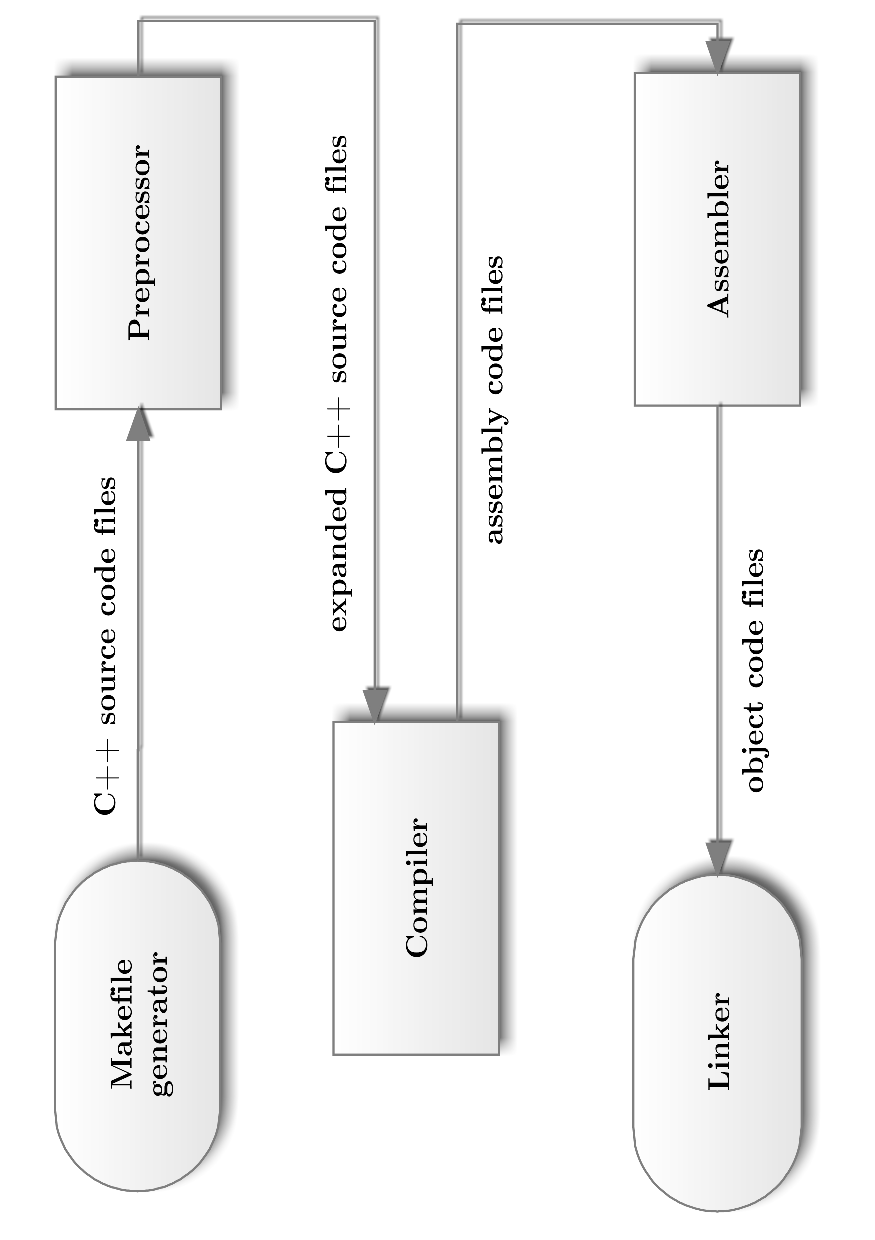
\includegraphics[angle=-90,width=11cm]{graphics/laboratory/09-classiccomp.pdf}
\caption{Classic \cpp{} code compilation process}\label{figure:classicpr}
\end{figure}

\fdocabbrevdeclare{moc}{moc}{Meta-object compiler}
\fdocabbrevdeclare{mos}{mos}{Meta-object system}
\section{Qt-way C plus plus compilation process}
Qt/\cpp{} compilation process (\autoref{figure:qtpr}) differs from classic \cpp{} code compilation process because \fdocabbrevref{moc}\index{meta-object compiler} comes into the compilation process. \fdocabbrevref{moc} one of fundamental basic stones of Qt itself. It is just more sophisticated preprocessor tool and source code generator. You will learn about \fdocabbrevref{moc} later becaus it is essential part of Qt \fdocabbrevref{mos}.

\begin{figure}[ht]
\centering
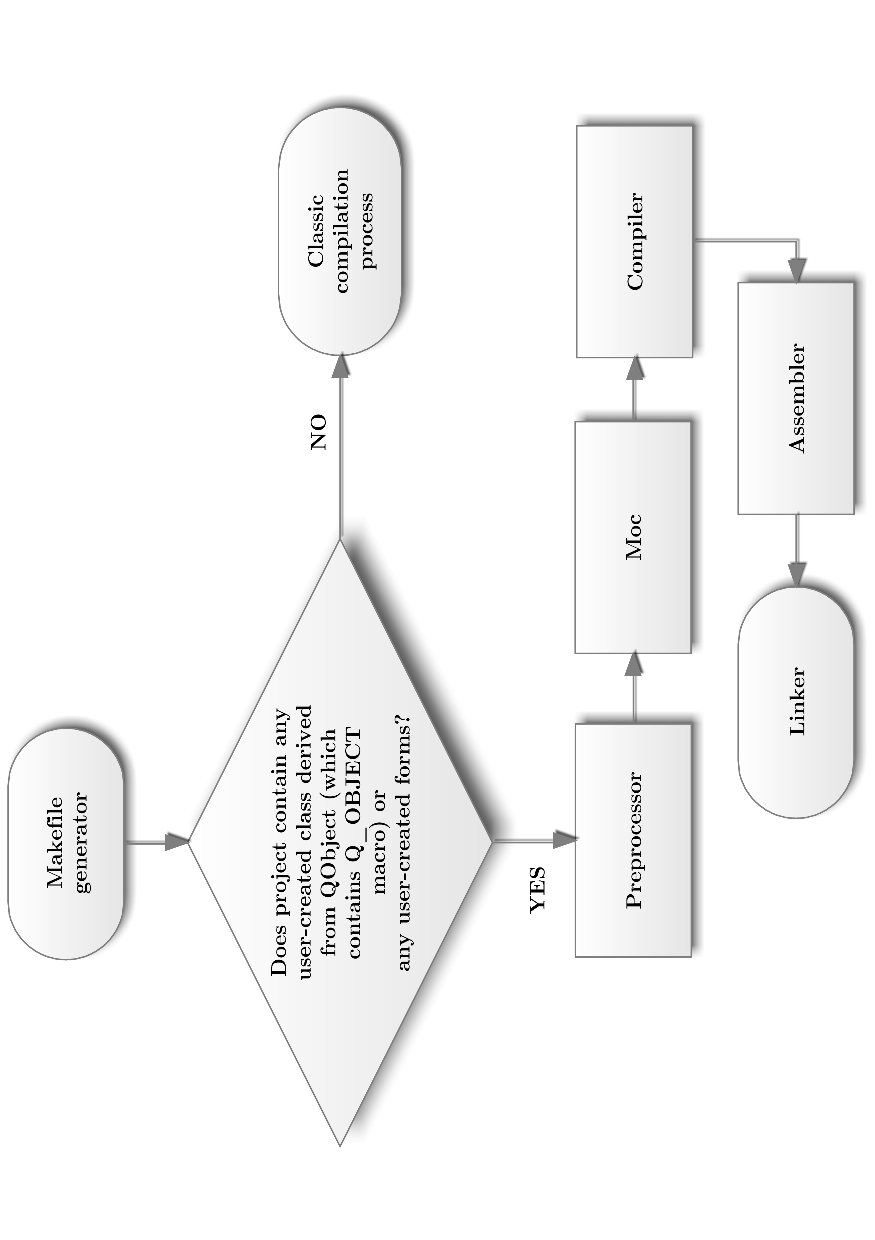
\includegraphics[angle=-90,width=14.5cm]{graphics/laboratory/10-qtcomp.pdf}
\caption{Qt-way \cpp{} code compilation process}\label{figure:qtpr}
\end{figure}

\chapter{Global Qt functions and macros}
Qt has its functionality separated into modules\index{module}. There is one special module (incarnated in QtCore module) called QtGlobal\index{QtGlobal}. QtGlobal is contained within single header file\fdocinlinecode{text}{!}{qglobal.h} and is the part of QtCore library file. QtGlobal contains following:
\begin{itemize}
\item
type clones (\autoref{table:types}) for every standard \cpp{} type,
\item
functions,
\item
macros.\index{macro}
\end{itemize}

\begin{table}[ht]
\begin{center}
\caption{\cpp{} type aliases in Qt}\label{table:types}
\begin{tabular}{c | c}
orignal type name & Qt type name \\
\hline
\fdocinlinecode{cpp}{!}{signed char} & \fdocinlinecode{cpp}{!}{qint8} \\ 
\fdocinlinecode{cpp}{!}{unsigned char} & \fdocinlinecode{cpp}{!}{quint8} \\ 
\fdocinlinecode{cpp}{!}{short} & \fdocinlinecode{cpp}{!}{qint16} \\ 
\fdocinlinecode{cpp}{!}{unsigned short} & \fdocinlinecode{cpp}{!}{quint16} \\ 
\fdocinlinecode{cpp}{!}{int} & \fdocinlinecode{cpp}{!}{qint32} \\ 
\fdocinlinecode{cpp}{!}{unsigned int} & \fdocinlinecode{cpp}{!}{quint32} \\ 
\fdocinlinecode{cpp}{!}{qint64} & \fdocinlinecode{cpp}{!}{qlonglong} \\ 
\fdocinlinecode{cpp}{!}{quint64} & \fdocinlinecode{cpp}{!}{qulonglong} \\ 
\fdocinlinecode{cpp}{!}{unsigned char} & \fdocinlinecode{cpp}{!}{uchar} \\ 
\fdocinlinecode{cpp}{!}{unsigned short} & \fdocinlinecode{cpp}{!}{ushort} \\ 
\fdocinlinecode{cpp}{!}{unsigned int} & \fdocinlinecode{cpp}{!}{uint} \\ 
\fdocinlinecode{cpp}{!}{unsigned long} & \fdocinlinecode{cpp}{!}{ulong} \\
\fdocinlinecode{cpp}{!}{double} & \fdocinlinecode{cpp}{!}{qreal}
\end{tabular}
\end{center}
\end{table}

\section{Fundamental functions}
QtGlobal offers very fundamental functions for value-based comparing and other basic tasks. These functions (often) wrap similar functions from standard C/\cpp library\index{standard library}. Most used functions are:
\begin{description}
\item[T qAbs(const T \& value)] \hfill \\
Returns absolute value of input parameter.
\item[const T \& qBound(const T \& min, const T \& value, const T \& max)] \hfill \\
Returns input value \enquote{rounded} to fit within bounds.
\item[double qInf()] \hfill \\
Returns value which represents infinity.
\item[qint64 qRound64(qreal value) and int qRound(qreal value)] \hfill \\
Mathematically rounds input paramater either to 64/32 bit integer.
\end{description}

All functons can be found in\fdocinlinecode{text}{!}{/qt-root-directory/include/QtCore/qglobal.h}. Some other functions will be used throughout the rest of the book.

\section{Producing console outputs with Qt}
Qt offers better way to produce console\index{console} printing for debugging purposes via \fdocinlinecode{cpp}{!}{QDebug}\index{QDebug} class and\fdocinlinecode{cpp}{!}{qInstallMessageHandler} function. You can always use traditional\fdocinlinecode{cpp}{!}{std::cout} for console printing but\fdocinlinecode{cpp}{!}{QDebug} way is much better. Basic syntax for using\fdocinlinecode{cpp}{!}{QDebug} is fairly simple (\autoref{listing:qdebug}) as it implements \fdocinlinecode{cpp}{!}{<<} operator and can act as \fdocinlinecode{cpp}{!}{printf(...)} function.

\begin{fdoccode}{cpp}{listing:qdebug}{Basic QDebug usage}
qDebug() << "Print this to standard output.";
qDebug("Print number %d.\n", 10);
\end{fdoccode}

First\fdocinlinecode{cpp}{!}{qDebug} usage requires explicit\fdocinlinecode{cpp}{!}{<QDebug>} inclusion. Second usage acts as wrapper for the\fdocinlinecode{cpp}{!}{printf} function from standard C library. You can use also\fdocinlinecode{cpp}{!}{qWarning},\fdocinlinecode{cpp}{!}{qCritical} or\fdocinlinecode{cpp}{!}{qFatal} functions according to importance of message.

Default implementation halts an application if\fdocinlinecode{cpp}{!}{qFatal} is called and uses\fdocinlinecode{cpp}{!}{std::cerr} output for printing messages. You can implement custom behavior for previous functions very simply:
\begin{enumerate}
\item
You need to implement global (or static) function with signature\fdocinlinecode{cpp}{!}{void (*function)(QtMsgType, const QMessageLogContext &, const QString &)}. Typical\\ implementation may look like \autoref{listing:qdebug2}.

\item
You need to assign handler to this function via\fdocinlinecode{cpp}{!}{qInstallMessageHandler} function.
\end{enumerate}

\begin{fdoccode}{cpp}{listing:qdebug2}{Typical printing handler for QDebug}
void debug_handler(QtMsgType type, const QMessageLogContext &placement, const QString &message) {
    switch (type) {
	case QtDebugMsg:
	    fprintf(stderr, "[%s] INFO (%s, line %d) : %s\n",
		    APP_LOW_NAME,
		    placement.file,
		    placement.line,
		    qPrintable(message));
	    break;
	case QtWarningMsg:
	    fprintf(stderr, "[%s] WARNING (%s, line %d) : %s\n",
		    APP_LOW_NAME,
		    placement.file,
		    placement.line,
		    qPrintable(message));
	    break;
	case QtCriticalMsg:
	    fprintf(stderr, "[%s] CRITICAL (%s, line %d) : %s\n",
		    APP_LOW_NAME,
		    placement.file,
		    placement.line,
		    qPrintable(message));
	    break;
	case QtFatalMsg:
	    fprintf(stderr, "[%s] FATAL (%s, line %d) : %s\nApplication is halting now.\n",
		    APP_LOW_NAME,
		    placement.file,
		    placement.line,
		    qPrintable(message));
	    qApp->exit(EXIT_FAILURE);
    }
}
\end{fdoccode}

Calling\fdocinlinecode{cpp}{!}{qFatal} function results in error dialog in Windows operating system (\autoref{figure:errordialog}).

\begin{figure}[ht]
\centering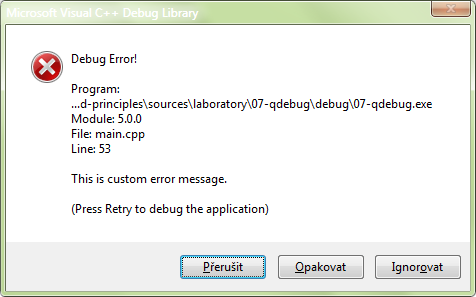
\includegraphics[width=9cm]{graphics/laboratory/11-debugdialog.png}
\caption{Application crash dialog in Windows}\label{figure:errordialog}
\end{figure}

\begin{fdocextra}
Debugging outputs should always be written in English language with ASCII character set.
\end{fdocextra}

This implementation prints out extra information which is extremely important for debugging. However, you can do whatever you want in your implementation. Storing outputs to database or sending them over network are just some possible enhancements.

The is another (simpler) way of forcing Qt to format console outputs if you want to tweak just format. You may tweak\fdocinlinecode{text}{!}{QT_MESSAGE_PATTERN} build environment variable to display application name or other useful information. Head to the documentation \citep{various:qtdoc} for more information.
%
%\subsection{Working with system environment variables}
%Major operating systems allow you to store data in the key--value pairs, so called environment variables.
\chapter{Meta-object system}
Meta-object system forms substantial part of Qt functionality, providing majority of Qt classes with ability to asynchronously report its state when something happens. Furthermore, you can equip even your custom classes with extra textual information, fetch names of your objects\index{object} at run time or make your classes use of the custom \textit{property system}\index{property system} that provides faster and syntactically unified access to your class member data.

\begin{fdocextra}
The word \enquote{meta} (which is originally Greek preposition, in Greek written as \enquote{\textmu \textepsilon \texttau \textalpha} was for the first time used by \textit{Aristotle}, the great Greek philosopher. Aristotle wrote plenty of writings, covering poetry, music or politics. His creations needed to be sorted later so that they could be interpreted correctly. Writings got sorted and scholars realized that there is one book with no name. It was placed \textit{after} Aristotle's great work \textit{Physics}. That's why that mysterious paper was named \textit{Metaphysics}, literally \enquote{the paper after Physics.}
\end{fdocextra}

\section{What is meta-object?}
Generally, meta-object is an entity that extends another object, providing us certain kind of information \textit{beyond} that particular object or set of objects. Meta-objects lie beyond actual objects, forming (kind of \enquote{higher}) abstraction layer of any Qt application. We can name this layer \textit{meta-echelon}\index{meta-echelon}.

Each class instance exposes its private data through \textit{methods} to its users -- other classes. Publicly available class members (methods or \textit{properties}\footnote{Property can be understood as private data member plus accessing getter/setter functions.}) form class interface, the only way to control class data and class behavior. This data is the only classical way to \enquote{see} the object from the view of its purpose but it says completely nothing about object inner structure and representation,\eg it doesn't expose type of on object (in run time) or count of its methods. Classic class methods do not provide us with \textit{meta-information}\index{meta-information}. Meta-objects do that.

\section{Reflection}
Ability to obtain and perhaps modify meta-information of any object is an action called \textit{introspection}\index{introspection} (or \textit{reflection})\index{reflection}. We can distinguish two kinds of reflection:
\begin{description}
\item[RUN TIME REFLECTION] \hfill \\
This is the superior way of reflection. Introspection of meta-information of certain object is possible at runtime but with one important addition. Compiler supporting run time reflection has absolutely no need to know the basis for meta-information construction at compile time. It does not need to add any extra data to the output code to allow reflection. Reflection is natural part of the language. This kind of reflection is supported primarily by languages that profit from using virtual machine\index{virtual machine} and special output executable file structure. Both Java and .NET-based languages (\eg \csharp or Visual Basic) provide this.
\item[COMPILE TIME REFLECTION] \hfill \\
Compiler of compile time reflection supported language has to do extra work to make reflection available. It usually produces extra code that grabs all (or most of) meta-information at compile time by going through the source code and extracting property names, method names, class names and other needed information. Extracted information is then formed into certain aggregations that are available as meta-objects at run time.

This approach makes the compilation little slower because an extra tool has to be executed to do the job. This concerns Qt. Qt uses meta-object compiler\index{meta-object compiler}\index{moc} to produce meta-objects.
\end{description}

\section{Qt meta-object system}
Qt uses compilation-based reflection\index{reflection} due to \cpp language limitations. Each object created within Qt meta-object system\index{meta-object system} is automatically equipped with shadow meta-object\index{meta-object}. This meta-object allows you to do amazing things with that particular object. You can obtain its class name, check if this object's class inherits another class, get name of the superclass\index{superclass} or names of its methods. You can even call methods by their names stored in a string (\autoref{listing:invoke})! Complete example can be found in\fdocinlinecode{text}{!}{sources/laboratory/08-invoke} directory.

\begin{fdoccode}{cpp}{listing:invoke}{String-based method invokation in Qt meta-object system}
#include <QDebug>

#include <iostream>

#include "myapplication.h"


int main(int argc, char *argv[]){
    MyApplication a(argc, argv);
    
    std::string input;
    qDebug("Type name of method to be executed: ");
    std::cin >> input;
    QMetaObject::invokeMethod(&a, input.c_str());

    return a.exec();
}
\end{fdoccode}

\section{Enabling meta-objectivity for custom classes}
Not all classes in a Qt-based application take part in the meta-object system. You need to to several steps to make sure that objects of your class will be accompanied with corresponding meta-objects:

\begin{enumerate}
\item Your class needs to inherit\fdocinlinecode{cpp}{!}{QObject}. Public inheritance is recommended.\fdocinlinecode{cpp}{!}{QObject} class is fantastic base stone for any custom classes in Qt application. You will learn about it in the next chapter.
\item Your class needs to contain\fdocinlinecode{cpp}{!}{Q_OBJECT} macro in its private section, best way is right under class name. This macro adds several methods to your class, one of them is all important\fdocinlinecode{cpp}{!}{QMetaObject *metaObject() const} method. Moreover, dynamic translation system is enabled by this macro too. You will learn about Qt applications translation later.
\end{enumerate}

\section{QObject class -- the cradle of meta-objects}
\fdocinlinecode{cpp}{!}{QObject}\index{QObject} class is the very base class for each meta-object-system-enabled class and provides many marvelous features. It is good to use\fdocinlinecode{cpp}{!}{QObject} as the base class even for your custom classes within any Qt application because there is one particularly amazing feature -- the automatic memory management provided by \nameref{section:model}.

\subsection{Qt object trees}\label{section:model}
There are some rules that apply to the way\fdocinlinecode{cpp}{!}{QObject} should be inherited. Copy constructor and assignment operator mustn't be implemented in inheriting class. Reasons are very simple:
\begin{enumerate}
\item Each and every\fdocinlinecode{cpp}{!}{QObject} instance stores pointer to its parent\fdocinlinecode{cpp}{!}{QObject} instance. This results in instance tree\index{tree hierarchy} hierarchy (\autoref{figure:modeltree}). Should copy of\fdocinlinecode{cpp}{!}{QObject} instance point to the parent of the original\fdocinlinecode{cpp}{!}{QObject} instance?

Consider situation in the \autoref{figure:samenames}. \enquote{George} instance was cloned and placed in the hierarchy. In general, there is no rule on where to place new copy in the tree hierarchy. It could be positioned as the sibling of the original object. New \enquote{George} is the sibling of the original \enquote{George}. Problem becomes clear when the original \enquote{George} instance is freed from memory. All its children are removed too, in other words, whole subtree with \enquote{George} as the root gets cleared from application memory but another (cloned) \enquote{George} remains untouched. Is this desired behavior? In some situations it could be but sometimes it's not.

\item Each\fdocinlinecode{cpp}{!}{QObject} instance has certain properties and those can be unique. Example of such a property is instance name (can be set by\fdocinlinecode{cpp}{!}{void	QObject::setObjectName(const QString & name)} function) which should be unique for each\fdocinlinecode{cpp}{!}{QObject} instance. The same name could be automatically assigned to the new copy of the instance but that results in two instances with the same name (\autoref{figure:samenames}) and that's the problem because you may want to search for one particular object by name which is possible in Qt. Two objects with the same name make search ambiguous.
\end{enumerate}

\begin{figure}[ht]
\centering
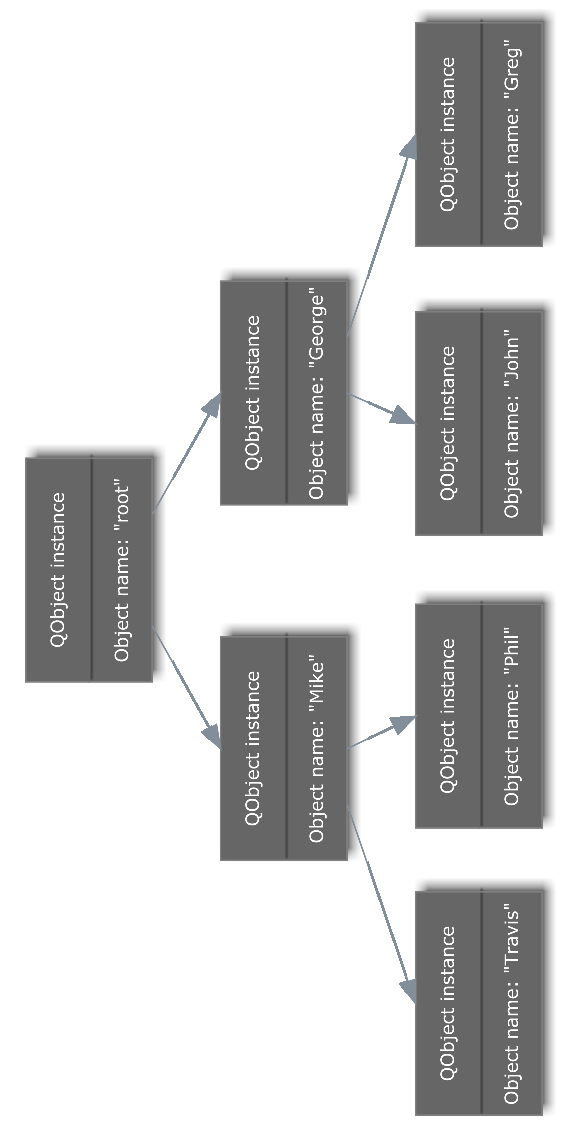
\includegraphics[angle=-90,width=13cm]{graphics/laboratory/12-modeltree.pdf}
\caption{QObject instances tree hierarchy}\label{figure:modeltree}
\end{figure}

\begin{figure}[ht]
\centering
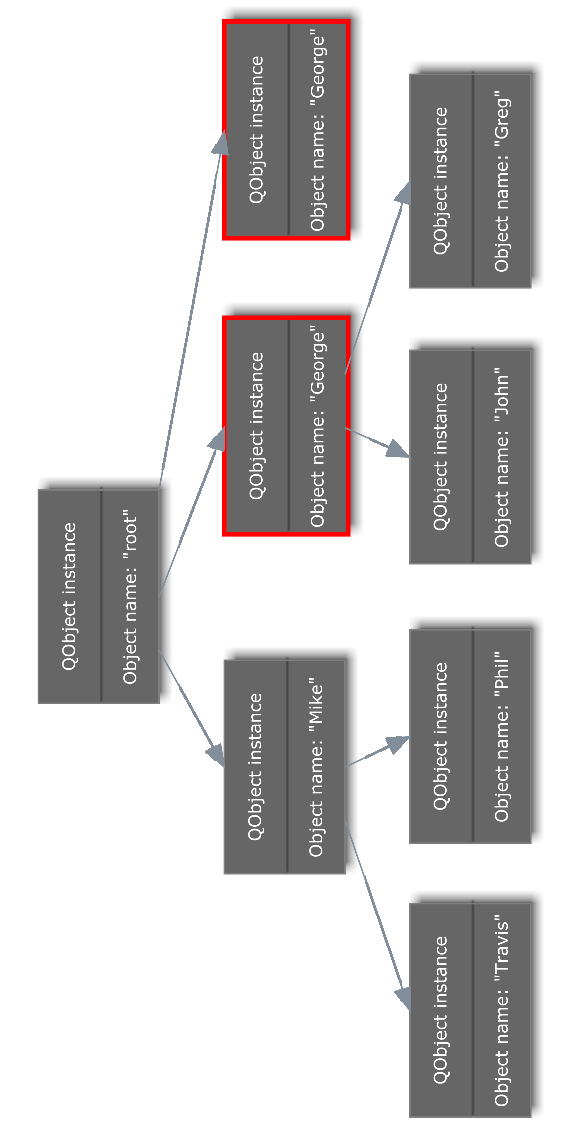
\includegraphics[angle=-90,width=13cm]{graphics/laboratory/13-samenames.pdf}
\caption{Broken QObject instances tree hierarchy}\label{figure:samenames}
\end{figure}

Every complex Qt-based application usually contains several\fdocinlinecode{cpp}{!}{QObject} tree hierarchies. These trees are disjunct. Example of typical tree hierarchy can be application main window. It usually contains menu bar, status bar, bunch of buttons, some text boxes and other visual elements. Naturally all these elements are owned by main windows. Thus, main window is the root of the main window elements tree hierarchy. If main windows is cleared from memory, then all its children are cleared from memory too which is desired behavior. This behavior makes memory management more automatic.

\indent\fdocinlinecode{cpp}{!}{QObject}-based object can be deleted from memory by calling\fdocinlinecode{cpp}{!}{this->deleteLater()} method or by using classic\fdocinlinecode{cpp}{!}{delete} operator. See more about deleting objects in Qt in \autoref{section:events}.

Existence of tree hierarchies impacts positively on several topics:
\begin{itemize}
\item more sophisticated memory management\footnote{Tree hierarchies form just part of Qt memory management as you will see in \autoref{section:memorym}.}
\item better track of the number of objects in application component
\item better debugging
\end{itemize}

\subsection{Subclassing QObject}
You have already read something about\fdocinlinecode{cpp}{!}{QObject} class in previous paragraphs. You know that\fdocinlinecode{cpp}{!}{QObject} instances form tree hierarchy. Subclassing\fdocinlinecode{cpp}{!}{QObject} is similar to standard \cpp class subclassing but you need to include\fdocinlinecode{cpp}{!}{Q_OBJECT} macro and you should instantiate\fdocinlinecode{cpp}{!}{QObject} with correct parent object, except some rare cases. Inheriting\fdocinlinecode{cpp}{!}{QObject} is very simple, just see \autoref{listing:qobjecti}.

You see that\fdocinlinecode{cpp}{!}{QObject} constructor accepts pointer to parent object which is used to construct\fdocinlinecode{cpp}{!}{QObject} base for\fdocinlinecode{cpp}{!}{MyQObject} instances.

\begin{fdoccode}{cpp}{listing:qobjecti}{Subclassing QObject}
/* header file (myqobject.h) */
class MyQObject : public QObject {
	Q_OBJECT
	
    public:
		explicit MyQObject(QObject *parent = 0);
};

/* source file (myqobject.cpp) */
#include "myqobject.h"


MyQObject::MyQObject(QObject *parent) : QObject(parent) {
}
\end{fdoccode}
%% případně ještě dynamic cast a QPointer a custom type.

\subsection{Signal--slot mechanism}
Signal--slot mechanism is the main tool to interconnect two \fdocinlinecode{cpp}{!}{QObject}-based objects, allowing thread-safe communication between them. Signals and slots form alternative to the callback mechanism. 

\begin{description}\label{desc:sig}
\item[What is signal?] \hfill \\
Signal is sign, which signs occurrence of specific event that happened during method execution of particular\fdocinlinecode{cpp}{!}{QObject}-based class. In fact, specially formed method with arbitrary number of arguments.
\item[What is slot?] \hfill \\
Slot is method in the same or another class which represents natural reaction to the signal occurrence.
\end{description}

\begin{figure}[ht]
\centering
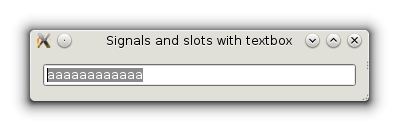
\includegraphics[width=8cm]{graphics/laboratory/14-ss-textbox.png}
\caption{Typical textbox example}\label{figure:ss-textbox}
\end{figure}

Imagine typical \textit{textbox}\index{textbox} control (\autoref{figure:ss-textbox}). This textbox could offers many \textit{signals} which are usual for this kind of control. Every textbox should emit appropriate signal if its content changes or if ENTER key is pressed by application user.

So there is textbox which emits signals. We need to have receiver of signals too. Receiver of signals from textbox could be for example the application. Application can perform some action (for example exit) if ENTER key is pressed inside textbox. Such an action is called \textit{slot}. If there exists slot in one particular entity that reacts to signals emitted by another entity, then we say that there is \textit{signal--slot connection} between these two entities.

One signal (of one entity) can be connected to several slots (contained in several entities), this behavior represents 1\text{:}N relationship. Several signals can be connected to one slot (M\text{:}1 relationship). Existence of 1\text{:}1 relationship is obvious.

Signal--slot mechanism does not apply just to \fdocabbrevref{GUI} elements. Every\fdocinlinecode{cpp}{!}{QObject} subclass can take advantage of it. Simple example can be file downloader class which signals progress of download.

\begin{fdocextra}
Tiny definitions of signal and slot on page \pageref{desc:sig} correspond with terms \index{event} and \index{delegate} known from .NET-based languages. \citep[p.~200-202]{nigel:csharp}
\end{fdocextra}

\subsubsection{Using signal--slot mechanism}
We are familiar with basic terms now. We are also able to subclass QObject. Let's implement very simple bank account representation. We expect that account provides us with possibility to save/withdraw money, check its status or make payments to another account.

Accounts are usually managed by bank. Bank ensures us that our payments are sent to the correct target accounts. Sample application can be found in\fdocinlinecode{text}{!}{sources/laboratory/11-bank} subdirectory. Let's dig into the application.

Application contains two primary classes:\fdocinlinecode{cpp}{!}{Account} and\fdocinlinecode{cpp}{!}{Bank}. Let's start with\fdocinlinecode{cpp}{!}{Account} class (see \autoref{listing:acc-head}). This class inherits\fdocinlinecode{cpp}{!}{QObject} (lines \ref{listing:qobj1}-\ref{listing:qobj2}), thus, meta-object features (including signal--slot mechanism) are available. Slots declaration is preceded by\fdocinlinecode{cpp}{!}{slots} keyword (line \ref{listing:slots1}) with any modifier. You can have public slot as well as private slot. It's just a matter of situation. As stated earlier, slot is just method with special behavior, it's able to react to signal occurrence.

Class \fdocinlinecode{cpp}{!}{Account} contains two signals. Their purpose is to inform connected\fdocinlinecode{cpp}{!}{QObject}-based instances (for example\fdocinlinecode{cpp}{!}{Bank} instances) about money flow within the account. Signals are placed in their own section (line \ref{listing:signals1}) preceded by\fdocinlinecode{cpp}{!}{signals} keyword.

\begin{fdocextra}
Quick look inside the Qt\fdocinlinecode{text}{!}{qglobal.h} file tells us that\fdocinlinecode{cpp}{!}{signals} keyword is synonym for\fdocinlinecode{cpp}{!}{public} keyword. Thus, signals are just public methods. This observation gets clarified on page \pageref{section:mocfun} in chapter \nameref{section:mocfun}.
\end{fdocextra}

\begin{fdoccode}{cpp}{listing:acc-head}{Account class design}
class Account : public QObject {(*@\label{listing:qobj1}@*)
	Q_OBJECT(*@\label{listing:qobj2}@*)

    public:
		// No copy constructor or assignment operator is declared,
		// just simple constructor.
		explicit Account(const QString &owner,
						int deposit,
						Bank *parent);

		// These are NOT slots.
		void status();
		QString name();

    public slots:(*@\label{listing:slots1}@*)
		// Used by customer who requests money from his account.
		// Customer can be either bank or account owner.
		void withdrawMoney(int sum);

		// Used by customer to save money to this account.
		// Customer can be either bank or account owner.
		void saveMoney(int sum);(*@\label{listing:slots2}@*)

    signals:(*@\label{listing:signals1}@*)
		// Emitted when money is withdrawn successfully from this account.
		void withdrawn(int sum);

		// Emitted when money is saved successfully into this account.
		void saved(int sum);(*@\label{listing:signals2}@*)

    private:
		QString m_owner;
		int m_deposit;
};
\end{fdoccode}

Second biggest class is the\fdocinlinecode{cpp}{!}{Bank} class (see \autoref{listing:bank-head}). Primary purpose of this class is to manage underlying accounts and make sure money transfers among them are okay.

\begin{fdoccode}{cpp}{listing:bank-head}{Bank class design}
class Bank : public QObject {
	Q_OBJECT

    public:
		explicit Bank(QObject *parent = 0);
		void printAccounts();
		void transfer(const QString &from, const QString &to, int sum);

    signals:
		// Emitted both accounts are ready for money transfer and
		// money should be withdrawn from the first account.
		void withdrawalWanted(int sum);

    protected:
		void checkAccounts();
		Account *getAccountByName(const QString &name);

    protected slots:
		void serveAccount(int sum);

	private:
		QList<Account*> m_accounts;

		Account *m_sendingAccount;
		Account *m_waitingAccount;
};
\end{fdoccode}

Money transfer is managed by\fdocinlinecode{cpp}{!}{void transfer(const QString &from, const QString &to, int sum)} method (\autoref{listing:bank-tran}). Method checks for existence of both accounts and some other tasks and, finally, establishes two signal--slot connections (lines \ref{listing:conn1}-\ref{listing:conn2}).

First connection says: \enquote{If bank wants to withdraw the money from the first account, then account must really withdraw the money.} Second connection says: \enquote{If the money was withdrawn from the first account, then bank should finalize money transfer by sending the money to the second account.}

Bank starts the money transfer procedure by trying to withdraw the money from the first account (line \ref{listing:conn3}).

\begin{fdoccode}{cpp}{listing:bank-tran}{Money transfer between accounts}
void Bank::transfer(const QString &from, const QString &to, int sum) {
    if (sum <= 0) {
		qDebug("You cannot transfer sum %d USD.", sum);
		return;
    }

    checkAccounts();

    Account *acc_from;
    Account *acc_to;
    if ((acc_from = getAccountByName(from)) == NULL) {
		qDebug("Source account is not registered in this bank.");
		return;
    }
    if ((acc_to = getAccountByName(to)) == NULL) {
		qDebug("Destination account is not registered in this bank.");
		return;
    }

    m_sendingAccount = acc_from;
    m_waitingAccount = acc_to;

    connect(this, &Bank::withdrawalWanted, acc_from, &Account::withdrawMoney);(*@\label{listing:conn1}@*)
    connect(acc_from, &Account::withdrawn, this, &Bank::serveAccount);(*@\label{listing:conn2}@*)

    emit withdrawalWanted(sum);(*@\label{listing:conn3}@*)
}
\end{fdoccode}

Money transfer gets done by serving the target account, which is done by calling method\fdocinlinecode{cpp}{!}{void serveAccount(int sum)}, but there still exists connection between the bank and the source account. This connection needs to be destroyed after the transfer completes so that another money transfer can be realized.

\subsubsection{Explanations}
We saw typical\fdocinlinecode{cpp}{!}{connect(....)} method usage on line \ref{listing:conn1} of \autoref{listing:bank-tran} it corresponds with this generic notation:
\begin{lstlisting}[firstnumber=1,language=cpp]
connect(source-object, source-signal, target-object, target-slot);
\end{lstlisting}
This is basic syntax for connecting two objects. First and third arguments are pointers to both objects. Second argument is signature of the source signal in the form\fdocinlinecode{cpp}{!}{&Class::signal}. Last argument is slot signature in the same form.

Both signal and slot have to have the same number of mutually compatible arguments which are passed to the slot when connected signal is emitted. Money sum was that argument in previous example.

There are other kinds of signal--slot connection. You can connect signal to another signal too:
\begin{lstlisting}[firstnumber=1,language=cpp]
connect(source-object, source-signal, target-object, target-signal);
\end{lstlisting}
Target signal is emitted when source signal is emitted. You can forward signals this way. This is primarily used in classes which form some kind of sublayer between to other layers which usually run in different threads.

\subsubsection{Signals and slots with regard to meta-object compiler}\label{section:mocfun}
There is a need of extra meta-object compiler job before the actual \cpp code compilation (see \autoref{figure:qtpr} on page \pageref{figure:qtpr}). \fdocabbrevref{moc} goes through every\fdocinlinecode{cpp}{!}{QObject}-based class in project and seeks signals and slots. If it founds any, then:
\begin{enumerate}
\item New source file is created, this file is named\fdocinlinecode{text}{!}{moc_original-name.cpp}. This file contains meta-information about all Qt entities from the original source file.
\item All signals are supplied with method bodies which are written to the\fdocinlinecode{text}{!}{moc_*.cpp} file.
\item Each slot/signal obtains unique integer id, starting from 0. So if class contains two signals and two slots, then their ids are $0,1,2,3$.
\end{enumerate}

Qt creates new meta-method which maps external method calls to signal/slot calls if signal is emitted or slot called. This mettod has signature\fdocinlinecode{cpp}{!}{int Account::qt_metacall(QMetaObject::Call _c, int _id, void **_a)} and its typical body looks like the one in \autoref{listing:qmetacall}. This code comes from Bank example, see\fdocinlinecode{text}{!}{sources/laboratory/11-bank}.

\begin{fdoccode}{cpp}{listing:qmetacall}{Signal/slot call entry point}
int Account::qt_metacall(QMetaObject::Call _c, int _id, void **_a)
{
    _id = QObject::qt_metacall(_c, _id, _a);
    if (_id < 0)
        return _id;
    if (_c == QMetaObject::InvokeMetaMethod) {
        if (_id < 4)(*@\label{listing:invoke2}@*)
            qt_static_metacall(this, _c, _id, _a);
        _id -= 4;
    } else if (_c == QMetaObject::RegisterMethodArgumentMetaType) {
        if (_id < 4)
            *reinterpret_cast<int*>(_a[0]) = -1;
        _id -= 4;
    }
    return _id;
}
\end{fdoccode}

This method is called if signal or slot of particular\fdocinlinecode{cpp}{!}{Account} instance should be invoked. Note that\fdocinlinecode{cpp}{!}{Account} offers two signals and two slots. Wanted operation checked in according to variable\fdocinlinecode{cpp}{!}{_c}. It states if signal/slot really needs to be invoked or if some other situation occurred. In our case, let's suppose that signal/slot should be called. Execution processes to line \ref{listing:invoke2}. Id of wanted element is checked on line and if id is less than four, then slot or signal is executed by\fdocinlinecode{cpp}{!}{void Account::qt_static_metacall(QObject *_o, QMetaObject::Call _c, int _id, void **_a)} method.

Signals and slots are compile time created entities but connections are not. There is no need to dig into technical aspects of connection. Generally, connection is collection of two pointers (source object and target object) and names of signals or slots. Signals and slots are invoked by name in run time. This was mentioned few pages back. Static method\fdocinlinecode{cpp}{!}{bool QMetaObject::invokeMethod(....)} is used to do that. \citep[QMetaObject class]{various:qtdoc}  You will learn something more about connections in chapter \nameref{section:thread} (page \pageref{section:thread}).


% TODO: použití lambda výratu
% TODO: property system

\subsection{QObject instance lifetime}
It's good to know something about events that happen during the life cycle of each and every\fdocinlinecode{cpp}{!}{QObject}-based instance.

\subsubsection*{Geniture}
\fdocinlinecode{cpp}{!}{QObject}-based object is born on the stack or on the heap. There is no real difference between stacked and heaped object from Qt perspective. New objects are added to one of trees (see \nameref{section:model} on page \pageref{section:model}) if they are created with valid parent pointer.

\subsubsection*{Lifetime}
Object is used as any other \cpp object/class. It can take part in many signal/slot connections.

\subsubsection*{Forfeiture}
Stacked objects are freed automatically if they are out of scope. This usually happens if method returns. Heaped objects are freed manually or by object tree destruction. All established connections are disconnected and signal\fdocinlinecode{cpp}{!}{void	destroyed(QObject *obj = 0)} is emitted just before object gets deleted from memory. You can connect other objects to this signal and delete them if signals occurs. You can chain several object trees this way.
\section{Memory management}\label{section:memorym}
Qt brings many new features into standard \cpp memory management. We can stick with plain\fdocinlinecode{cpp}{!}{new} and\fdocinlinecode{cpp}{!}{delete} operator. Qt features are, however, highly addictive and useful. We have already heard about object trees (page \pageref{section:model}) which are real base for Qt memory management because tree structure is quite natural. Therefore, object trees are used much and many memory leaks is fixed with them.

Each object tree has root object and we (as programmers) are responsible for deleting this root from memory in the right time as there is no other parent object which gets this done for us.

\subsection{Copy-on-write}
Qt uses copy-on-write\index{copy-on-write} technique for managing Qt classes data. If you copy\fdocinlinecode{cpp}{!}{QString} instance, then these two instances point to the same textual data, unless you try to modify contents of any instance. Shared data are then copied to new place and each instance has its own data. Modifications are done after. 

\subsection{Safe pointers}
Pointers are both great and evil. They offer us great possibilities, \eg they are used as thin method parameters. Pointers are also cause of the most of application crashes. We often use pointers which point to 0. Qt offers better pointers. They deal with their invalidity and ensuring that pointer is used only if it points to existing object. Lets introduce\fdocinlinecode{cpp}{!}{QPointer} class. \citep[QPointer class]{various:qtdoc}

\fdocinlinecode{cpp}{!}{QPointer} does one simple job, it sets pointer to 0 if it's deleted. This helps a lot because you can check if pointer is valid by comparing it to 0. This class is pretty straightforward, look at documentation for more information.
\chapter{Event system}\label{section:events}
Events do not  Generally, events are reactions for some other actions. In software, actions can be divided into to categories:
\begin{description}
\item[HUMAN-TRIGGERED ACTIONS] \hfill \\
This type of actions represents natural notion of what events are. Mouse button clicks, keyboard key presses or perhaps cursor movements are human-triggered events. Each of them disposes certain properties, \eg mouse-click produces coordinates of click or key push produces the pressed character or perhaps set of characters if key sequence is used.
\item[APPLICATION-TRIGGERED ACTIONS]  \hfill \\
Are not triggered directly by application user. Typical application-triggered event is painting event which is responsible for drawing \fdocabbrevref{GUI} elements on the screen. User starts this event indirectly by manipulating application user interface.
\end{description}

Event is consequence of occurrence of certain action in running application. There are plenty of various types of events. Typical event might be key-press-event or perhaps mouse-click-event or repaint-gui-event.

Each\fdocinlinecode{cpp}{!}{QObject} subclass has ability to send events. Events are usually distributed by one entity which manages whole event process. This entity \enquote{sits} on the top of event loop. Event loop is part of application execution which encapsulates all events sent by objects inside the loop. Loop goes from time to time through all raised events from its underlying objects and delivers those events to target objects. Event loop structure looks similar to one in \autoref{listing:eventloop2}. Event loop exits if \enquote{exit} signal occurs.

Each Qt application has one main global event loop with\fdocinlinecode{cpp}{!}{QApplication} instance as managing entity (entity which caused the creation of the event loop). Consider \autoref{listing:eventloop}. Call on line \ref{listing:loop1} of \autoref{listing:eventloop} results in entering to global event loop, so that events from application objects, \eg from main application window, can be processed.


\begin{fdoccode}{cpp}{listing:eventloop}{Global event loop}
int main(int argc, char *argv[]) {
    QApplication a(argc, argv);
    
    // Display main application window here.
    .............

	// int QApplication::exec() triggers global event loop.
    return a.exec();(*@\label{listing:loop1}@*)
}
\end{fdoccode}

\begin{fdoccode}{cpp}{listing:eventloop2}{Typical event loop structure}
while() {
	if (exit) {
		return status;
	}
	check_queue_of_pending_events;
	process_all_pending_events;
	remove_processed_events_from_the_queue;
}
\end{fdoccode}

\begin{figure}[ht]
\centering
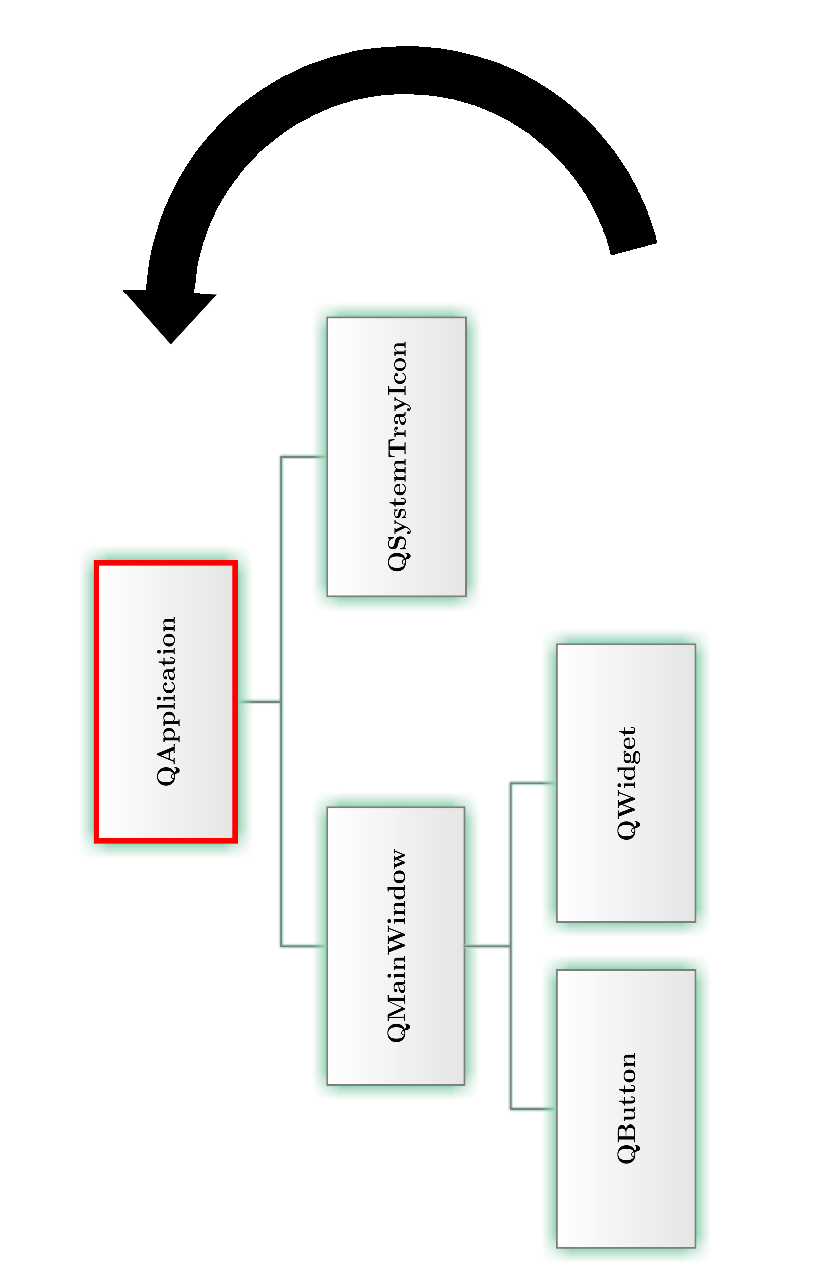
\includegraphics[angle=-90,width=11cm]{graphics/laboratory/15-eventloop.pdf}
\caption{Typical event loop}\label{figure:eventloop}
\end{figure}

Let's take a look at \autoref{figure:eventloop} which displays typical structure of Qt application.  Arrow indicates position of supervising entity (entity which triggered event loop). If\fdocinlinecode{cpp}{!}{QSystemTrayIcon} notices that certain event happened in it,\fdocinlinecode{cpp}{!}{QApplication} instance is notified about the situation and is given information about:
\begin{itemize}
\item type of event
\item event properties
\item sender
\end{itemize}
Event (object) is posted by\fdocinlinecode{cpp}{!}{QSystemTrayIcon} and appended to event loop queue for further processing and\fdocinlinecode{cpp}{!}{QSystemTrayIcon} possibly waits for backward event delivery from event loop.

\indent\fdocinlinecode{cpp}{!}{QApplication} event loop iterates and finds new unsolved events which are eventually removed from the queue and sent to their senders.\fdocinlinecode{cpp}{!}{QSystemTrayIcon} then \textit{handles} the event and responds with expected behavior which finally concludes life of this event.

Handling event means calling \textit{event handler} -- some kind of special method. If you handle some events in one object, sometimes you need to \textit{propagate} the same event in another object too. For example if you move use\fdocinlinecode{cpp}{!}{QButton} (ordinary button) instance by mouse, then paint-event is raised, because\fdocinlinecode{cpp}{!}{QButton} needs to be repainted on the screen, and this event is propagated to parent object which is usually application window which needs to redraw itself too. Some events are propagated and other ones are not.

Easiest way to handle events in Qt is reimplementing available event handlers. Each\fdocinlinecode{cpp}{!}{QObject} offers specific handlers. All handlers are declared as protected methods. See \autoref{listing:reimplm} (example\fdocinlinecode{text}{!}{sources/laboratory/12-child-event}) for typical extension of event handler. In this case, we reimplemented behavior of child-event which is triggered if child is added or removed to particular\fdocinlinecode{cpp}{!}{QObject} instance. Event handler of superclass is called on line \ref{listing:handl} because we want to only extend the original handler and not to replace its behavior completely. This approach is common in Qt and is used especially for \fdocabbrevref{GUI}-related events.

\begin{fdoccode}{cpp}{listing:reimplm}{Reimplementing event handler}
// myqobject.h
class MyQObject : public QObject{
	Q_OBJECT

    public:
		explicit MyQObject(QObject *parent = 0);

    protected:
		void childEvent(QChildEvent *event);
};

// myqobject.cpp
#include <QChildEvent>

#include "myqobject.h"


MyQObject::MyQObject(QObject *parent) : QObject(parent) {
}

void MyQObject::childEvent(QChildEvent *event) {
    if (event->added()) {
		qDebug("Child %s (%s) was added to %s.",
	       	event->child()->metaObject()->className(),
	       	qPrintable(event->child()->objectName()),
	       	qPrintable(objectName()));
    }
    else if (event->removed()) {
		qDebug("Child %s (%s) was removed from %s.",
	       	event->child()->metaObject()->className(),
	       	qPrintable(event->child()->objectName()),
	       	qPrintable(objectName()));
    }

    QObject::childEvent(event);(*@\label{listing:handl}@*)
}
\end{fdoccode}

% TODO: 
% metoda QObject::startTimer...událost dále customEvent
% diagram cyklu
% deleteLater vs delete
% qapplication event loop

\section{Event filters}
Classic event handlers maybe unusable if you want to handle all events in one place. One solution is to use generic\fdocinlinecode{cpp}{!}{bool QObject::event(QEvent * e)} event handler which catches all events. Another solution of this approach is event filtering. Event filter is ordinary method which accepts destination\fdocinlinecode{cpp}{!}{QObject} instance and event object. Example (\autoref{listing:reimplm2}) shows the approach quite clearly.

\begin{fdoccode}{cpp}{listing:reimplm2}{Using event filter}
// myqobject.h
class MyQObject : public QObject {
	Q_OBJECT

    public:
		explicit MyQObject(QObject *parent = 0);

    protected:
		bool eventFilter(QObject *object, QEvent *event);
};

// myqobject.cpp
#include <QEvent>

#include "myqobject.h"


MyQObject::MyQObject(QObject *parent) : QObject(parent) {
    installEventFilter(this);
}

bool MyQObject::eventFilter(QObject *object, QEvent *event) {
    qDebug("Event happened in %s.", qPrintable(object->objectName()));

    if (event->type() == QEvent::ChildAdded) {
	qDebug("Observing child-event for %s and child %s.",
	       qPrintable(object->objectName()),
	       qPrintable(static_cast<QChildEvent*>(event)->child()->objectName()));
    }

    return QObject::eventFilter(object, event);
}
\end{fdoccode}


% TODO: Custom events.
%\subsection{Custom events}

% TODO: QObject timers
%\subsection{QObject timers}
\chapter{Threading}\label{section:thread}
Every modern and flawless application needs to superimpose its functionality into several layers. One layer often represents \fdocabbrevref{GUI}, while another takes care of storing application data in a database or provides some kind of extensive mathematical computations. Dividing application functionality into separated blocks is a good approach. Paramount technique for this approach is called \textit{threading}\index{threading}.

\section{What is thread?}
Operating system has only one duty\,--\,it must allow client programs to run. But programs cannot run simultaneously, so only one program is run at a time and other programs are forced to wait until it's their turn. They are patiently waiting in the queue for their chance to become active and do the job they are asked to do. 

Operating system allocates very tiny amount of time for each program and switches among them very swiftly. Each program usually lives for several milliseconds in one round. This circling among programs (sometimes called \textit{processes}\index{process}) is called \textit{multitasking}\index{multitasking}.

Moreover, every program can be divided into several parts which can run independently. Operating system, in fact, cycles among these program parts instead of whole programs. Independently-runnable part of the program can be called \textit{thread of execution}\index{thread}. Each and every computer program contains at least one thread. Important thing about threads is that all threads of one process share its resources\,--\,joint data. Shared data allows you to make your threads cooperate with each other. Threads are used for many purposes:
\begin{description}
\item[COMMUNICATION] \hfill \\
Threads are used to handle communication among entities like web servers or other remote devices.
\item[INTERFACE LATENCY] \hfill \\
If you do not separate extensive computations from your \fdocabbrevref{GUI} then \fdocabbrevref{GUI} may be blocked when those computations are performed. Threads are used to separate computations from GUI. Interface thread is no longer blocked by computations and no freezing occurs.
\item[PARALLEL COMPUTING] \hfill \\
Certain formulas are very difficult to solve in reasonable time and the only way to make computations faster is to make them running collaterally.
\item[GOOD HABIT] \hfill \\
Experienced programmer always tries to divide application functionality into well-formed and rationally-built parts. Threading is great and powerful technique to achieve that.
\end{description}

\fdocabbrevdeclare{PThreads}{PThreads}{POSIX Threads}
\section{Threading and operating system}
Threading was added to some operating systems additionally. The only way to do that was via library. This was the case of \fdocabbrevref{PThreads} on Linux. Threads were not part of the official Linux concept and became available later.

\section{Threading in Qt}
\fdocabbrevref{PThreads} library is used as the backend for Qt threading support on Linux and Windows. Threading is very complicated and complex subject but at least basic usage (which is fine for most users) can be introduced.

Base class for working with threads is\fdocinlinecode{cpp}{!}{QThread}. \citep[QThread class]{various:qtdoc}  \fdocinlinecode{cpp}{!}{QThread} should \textbf{never} be subclassed. If you want to run code of any class in separated thread, then you need to:
\begin{enumerate}
\item Derive your class from\fdocinlinecode{cpp}{!}{QObject} and add signals/slots of your desire to it.
\item Create new\fdocinlinecode{cpp}{!}{QThread} instance.
\item Call\fdocinlinecode{cpp}{!}{void QObject::moveToThread(QThread *targetThread)} with your class as\fdocinlinecode{cpp}{!}{this} pointer.
\end{enumerate}

There is no need to do this procedure for static methods or global functions. You can use\fdocinlinecode{cpp}{!}{QFuture<T> QtConcurrent::run(void *function)} to run those. \citep[QtConcurrent]{various:qtdoc} See \autoref{listing:qtconc} (example\fdocinlinecode{text}{!}{sources/laboratory/14-threading}) for more.

\begin{fdoccode}{cpp}{listing:qtconc}{QtConcurrent usage for global or static functions}
void faktorial(int input) {
    qDebug().nospace() << "Factorial from thread " << QThread::currentThreadId() << ".";

    if (input < 0) {
		return;
    }

    int result = 1;
    for (int i = 1; i <= input; i++) {
		result *= i;
    }

    qDebug() << result;
}


int main(int argc, char *argv[]) {
    QCoreApplication a(argc, argv);

    // Number of main thread handle?
    qDebug() << "Main thread is " << QThread::currentThreadId() << ".";

    // Use QtConcurrent for glogal function.
    QFuture<void> result = QtConcurrent::run(faktorial, int(5));
    result.waitForFinished();

    return a.exec();
}
\end{fdoccode}

Advance usage of threading is introduced in part \nameref{part:real}.
%% vlákna - Qt::QueuedConnection - propojení se signály a sloty
%% gui
%% rss guard

\realworld
\part{Real-world Qt}\label{part:real}
\pagestyle{fancy}
\chapter{Foreword}

\section{What is covered in this part?}
This part is different from the previous one. In this part, you will be guided through development of more complex Qt-based application. Important parts of development process will be discovered, including initial ideas, solving dependencies, licensing, programming the application, translating or publishing.

Someone could state that licensing issues or publishing the application is not important. Programmer's main task is to program the application correctly.\ That's true but programmer needs to take advantage of other tasks too because all of them provide him with chance of producing event better software.

There is quite good documentation \citep{various:qtdoc} available for Qt but it lacks some parts which are covered in this part of the book. We will see how to automatically build our software with needed customizations or how to make our software available to users.

\section{Lifecycle of typical application}
Development of typical application starts if someone needs something. Photographer wants special photo-editing software which doesn't seem to be available. Or perhaps teacher needs to have specific agenda application for his particular needs. Programmers often program new software for themselves. So applications are born due to various (and usually rational) reasons.

Before the application is actually written, there must be certain research done by the programmer. See \autoref{chap:new} for more about this topic. Special \enquote{50:50} rule applies here. It's unwritten rule that you (as the programmer) should spent at least $50\%$ of your time (dedicated for development of particular software) for research. You should think about problems and choose right algorithms. The other $50\%$ is meant to be time for writing your ideas in programming language. Most huge failures roots in shoddy research.

\chapter{Creating new applications}\label{chap:new}
There is usually need for something useful in the beginning. Sample application for this book is the same case. It is called Qonverter and it is supposed to be very simple calculator with some unusual functions and features.

Some time ago, i needed calculator with ability to do some more advanced (but still simple) operations. I needed to compute factorials or medians. I also needed to do bitwise operations on numbers such as shifting or logical conjunctions and disjunctions along with usual mathematical operations. Moreover, I needed to do unit and currency conversions sometimes.

I searched for calculator application which could offer such a functionality to me. No satisfying results were found. Unit (currency) converter was usually missing. Many calculators doesn't offer specific mathematical functions I like to use from time to time.

So I decided to write my own calculator which provides function I need.

\section{Choosing programming language}
I am not skilled programmer but i know \cpp{} programming language, so it was easy to choose. Anyway, choice of programming language is extremely important. You may take a look at section \nameref{subsection:cpp} to see \cpp{} features. \cpp{} is fairly fast so it is good choice for this kind of application.

I decided to use newest (as of January 2013) \cpp{} version called \cpp{} 11. It offers many features (some already mentioned in this book) which can bring me many advantages:
\begin{itemize}
\item shorter code,
\item easier-to-understand code,
\item (perhaps) greater performance.
\end{itemize}

Many disadvantages can arise:
\begin{itemize}
\item lack of support by \cpp{} compilers,
\item lack of support by libraries.
\end{itemize}

\fdocabbrevdeclare{MinGW}{MinGW}{Minimalistic GNU for Windows}
There are many \cpp{} compilers to choose from. I want to keep my Qonverter multiplatform because I use both Linux and Windows operating systems. \fdocabbrevref{GCC} is main compiler for Linux, so there is clear situation. Latest \fdocabbrevref{GCC} (version 4.8.0, as of March 2013) is known to support all major features of \cpp{} 11. Several great compilers are available for Windows platform. I could use \fdocabbrevref{MSVC} 2010 compiler but it lacks some \cpp{} 11 features so latest \fdocabbrevref{MinGW} compiler was chosen instead. \fdocabbrevref{MinGW} is \fdocabbrevref{GCC}-based compiler. Mac OS X operating system uses Clang compiler which is known to support \cpp{} 11 too \citep{various:clang}. So hypothetically, these operating systems might be supported:
\begin{itemize}
\item Windows,
\item GNU/Linux,
\item Mac OS X.
\end{itemize}
In fact, even more operating systems can be supported in the future, because Qt is ported for example to eComStation \citep{various:ecomstation} operating system.


\section{Choosing libraries}
I picked compilers and programming language in five minutes. It wasn't the big deal. I had to choose libraries too and that was the big deal. I knew just few libraries but only one which provides me with ability to build \fdocabbrevref{GUI}. It was Qt. Latest Qt (Qt 5) is known to work with \cpp{} 11. It just came out when i decided to create Qonverter (spring of 2012) so I decided to use it.

One last piece of puzzle needed to be found. Library for mathematical core of the application. I was searching for the right one for one week and nothing great appeared. Eventually, I discovered muParserX library \citep{various:muparserx}.

%\upendoftreatise
%\fdocendofmainmatter
%\fdocappendix
%\section{First cute appendix}
%Whatever\ldots


\upendoftreatise

\upprintlists

\fdocendofmainmatter

\fdocprintbibliography
\fdocprintindex

\end{document}